\documentclass[12pt,a4paper]{article}

\usepackage[onehalfspacing]{setspace}
\usepackage{natbib}
 
\usepackage{float}
%f�r feststellen der figures und tables [H] dranschreiben
\usepackage{siunitx}
%\SI{value}{unit commands} \SI{value}[pre-unit]{unit commands}
%\usepackage{units}
%wird so benutzt: 
%\unit[value/Zahl]{dimension/Einheit} oder 
%\unitfrac[value/Zahl]{dimension/Einheit num/Z�hler}{dimension/Einheit denum/Nenner} oder
%\nicefrac[fontcommand/Schriftart]{dimension/Einheit num/Z�hler}{dimension/Einheit denum/Nenner}
\usepackage{amssymb}
\usepackage{caption}
\usepackage{subcaption}

\usepackage{hyperref}

\usepackage[left=2cm,right=2cm,top=2cm,bottom=2cm]{geometry}
\usepackage[latin9]{inputenc}
\usepackage[ngerman]{babel}
\usepackage[T1]{fontenc}
\usepackage{lmodern}
\usepackage{amsmath}
\usepackage{graphicx}
\usepackage{textcomp}



\begin{document}

%deckblatt erstellen.

\begin{titlepage}

\begin{center}
% Oberer Teil der Titelseite:

\includegraphics[width=0.75\textwidth]{logo.png}\\[1cm]    	%Logo 

\textsc{\LARGE Bergische Universit\"at Wuppertal}\\[1.5cm]	%Institution

\textsc{\Large Fortgeschrittenen Praktikum}\\[0.5cm]				%Projekt


\newcommand{\HRule}{\rule{\linewidth}{0.5mm}}
\HRule \\[0.4cm]
{ \huge \bfseries Rutherford\\ Streuung von $\alpha$-Teilchen}\\[0.4cm]				%Titel

\HRule \\[1.5cm]

% Author und Tutor
\begin{minipage}{0.4\textwidth}
\begin{flushleft} \large
\emph{Verfasser:}\\
Henrik \textsc{J�rgens} \\
Frederik \textsc{Strothmann} \\
\end{flushleft}
\end{minipage}
\hfill
\begin{minipage}{0.4\textwidth}
\begin{flushright} \large
\emph{Tutoren:} \\
Max \textsc{Mustermann} \\
Max \textsc{Mustermann} \\
\end{flushright}
\end{minipage}

\vspace{1cm}

\begin{table}[H]
\centering
\begin{tabular}{|l|}
\hline \textbf{Abstract: } \\
Ziel des Versuches ist es, die Wechselwirkung von $\alpha$-Teilchen mit Materie zu untersuchen.\\
Die Aspekte Streuwinkel, Reichweite, Kernladung und Absorbtionsverhalten werden thematisiert.\\
\hline 
\end{tabular}
\end{table} 

\vspace{1cm}

\begin{table}[H]
\centering
\begin{tabular}{|c|c|c|}
\hline Dies & ist & ein \\ 
\hline Platz- & halter & f�r \\ 
\hline die & bewertungs & Tabelle \\ 
\hline 
\end{tabular} 
\end{table}

\vfill

% Unterer Teil der Seite/Datum
{\large \today}

\end{center}

\end{titlepage}

\newpage
\tableofcontents
\newpage

\bibliographystyle{plain}


\section{Einleitung}
%einleitung zu dem experiment.
%auf die einstellungen, die vor dem versuch gemacht werden, eingehen, oder auf eine anleitung dazu verweisen.
%---------------------------------------------------------------------------------------------
%hinter der einleitung kann der allgemeine theoretische hintergrund in einer zus�tzlichen section erkl�rt werden
In diesem Versuch werden Oberfl�chen verschiedener Proben mittels Rasttunnelmikroskopie auf deren Gitterstruktur und morphologische Eigenschaften untersucht. Elektronendichte, Oberfl�chenrauheit und die atomare Gitterstruktur k�nnen mit dem Rastertunnelmikroskop (RTM) analysiert werden. Der quantenmechanische Tunneleffekt wird genutzt, um leitende Materialien zu untersuchen. Indem zwischen einer einatomigen Platin-Iridum-Elektrode und der zu untersuchenden Probe eine Potentialdifferenz angelegt wird, kommt es abh�ngig von der Entfernung der Pt-Ir-Elektrode zur Probe und dessen Elektronendichte zu einem Tunnelstrom, welcher R�ckschl�sse auf die Struktur der Probe erlaubt. Die Elektronendichte der Oberfl�che kann durch systematisches Abrastern der Probe erfasst werden, sodass mithilfe verschiedener Modi (CC und CH: Constant Current und Constant Height) ein Bild der Materialoberfl�che entsteht.
\section{Theorie}
% Es sollen die wichtigsten theoretischen Formeln und Zusammenh�nge einmal ausf�hrlich erkl�rt werden
Es werden die theoretischen Grundlagen zur Bestimmung der Lebensdauer von Myonen besprochen.

\subsection{Standardmodell}
Das Standartmodell der Teilchenphysik drei der vier Grundlegenden Wechselwirkungen (WW), die schwache WW, die elektromagnetische WW und die Starke WW.
Die Kr�fte wechselwirken �ber Vektorbosonen, welche eine ganzzahligen Spin haben.
In Tabelle \ref{tab:ww} ist eine �bersicht der drei Kr�fte zu sehen.

\begin{table}[H]
\caption{In der Tabelle sind die Grundlegenden WW (au�er der Gravitation) und ihre Eigenschaften aufgetragen (entnommen \cite{povh} Seite 274)}
\label{tab:ww}
\centering
\begin{tabular}{|c|c|c|c|c|}
\hline Wechselwirkung & koppelt an & Austauschteilchen & $\frac{m_0}{GeV}$ & J$^P$ \\ 
\hline stark & Farbe & 8 Gluonen (g) & 0 & 1$^-$ \\ 
\hline elektromagnetisch & elektrische Ladung & Photon ($\gamma$) & 0 & 1$^-$ \\ 
\hline schwach & schwache Ladung & W$^\pm$, Z$^0$ & $\approx 10^2$ & 1 \\ 
\hline 
\end{tabular} 
\end{table}
Neben den Bosonen gibt es noch zwei weitere Fundamentale Teilchenarten die Quark und die Leptonen welche die Grundbausteine der Materie darstellen.
Beide geh�ren zu den Fermionen, haben also einen halbzahligen Spin. Leptonen und Quarks werden mit aufsteigender Masse in drei Generationen aufgeteilt.
In Tabelle \ref{tab:fermi} sind Quarks und Leptonen mit ihren Eigenschaften dargestellt.

\begin{table}[H]
\caption{�bersicht der Grundlegenden Eigenschaften von Quarks und Leptonen}
\label{tab:fermi}
\centering
\begin{tabular}{|p{2cm}|p{2cm}|p{2cm}|p{1cm}|p{3.5cm}|p{1cm}|}
	\hline
	Fermionen & \hspace{0.25cm} Familie \newline 1 \hspace{0.3cm} 2 \hspace{0.3cm} 3                                               & elektrische Ladung    & Farbe  & schwacher Isospin \newline rechtsh. \hspace{0.5cm} linksh. & Spin \\ \hline
	Leptonen  & $\nu_e$ \hspace{0.17cm} $\nu_\mu$ \hspace{0.17cm} $\nu_\tau$ \newline e \hspace{0.3cm} $\mu$ \hspace{0.3cm} $\tau$ & \hspace{0.6cm} 0 \newline  \hspace*{0.6cm} -1      & ------ & 1/2 \hspace{1.5cm} --- \newline \hspace*{2.4cm} 0          & 1/2  \\ \hline
	Quarks    & u \hspace{0.3cm} c \hspace{0.3cm} t \newline d \hspace{0.3cm} s \hspace{0.3cm} b                                   & \hspace*{0.2cm} +2/3 \newline \hspace*{0.3cm} -1/3 & r,g,b  & 1/2 \hspace{1.64cm} 0 \newline \hspace*{2.4cm} 0           & 1/2  \\ \hline
\end{tabular} 
\end{table}


\section{Messung des Emissionsspektrums}
%kurz das ziel dieses versuchsteiles ansprechen, damit keine zwei �berschriften direkt �bereinander stehen!
%bei schwierigeren versuchen kann auch der theoretische hintergrund erl�utert werden. (mit formeln, herleitungen und erkl�rungen)
Im ersten Versuchsteil wird das R�ntgenspektrum der Kupferanode mit einem Silicium(111)-Einkristall untersucht, f�r die Untersuchung werden drei verschieden Beschleunigungsspannungen und ein Ni-Filter verwendet. Untersucht werden die Z�hlraten in Abh�ngigkeit des Winkels, sowie die Lage aller Ordnungen der K$_{\alpha_{1,2}}$- und K$_\beta$-Linien von Kupfer und deren Verh�ltnisse. Dann wird das Signal-Rausch-Verh�ltnis untersucht und weitere Details der Spektren besprochen. Im Anschluss werden die Netzebenabst�nde anderer Einkristalle untersucht. Untersucht werden Si(331)- und Ge(111)-Einkristalle. Die bestimmten Netzebenabst�nde werden mit Literaturwerten abgeglichen.

%Versuchsdurchf�hrung
\section{Versuchsdurchf�hrung}
%erkl�ren, !was! wir machen, !warum! wir das machen und mit welchem ziel
%(wichtig) pr�zize erkl�ren, wie bei dem versuch vorgegangen und was gemacht wurde
\subsection{Hochspannung der Photomultiplier}
Ein exaktes einstellen der Photomulitplier ist ist essenziell f�r eine gute Messung. Die Spannungen von PM1, PM2 und PM4 sollen dabei einen Wert von 2100 V nicht �berschreiten. Der Arbeitspunkt von PM3 liegt im Bereich von 2600-2700 V. F�r die Bestimmung des optimalen Arbeitspunktes wird die Schwelle des Diskriminators auf einen m�glichst geringen Wert eingestellt. Es wird die die Z�hlrate in Abh�ngigkeit der Spannung untersucht und nach einem  Plateau im Bereich von 100 bis 1000 Counts/s gesucht, da sich der Photomulitplier dann am optimalen Arbeitspunkt befindet. Falls die Z�hlraten zu niedrig sind kann ein $^{60}Co$-Pr�parat verwendet werden, um die Z�hlrate zu erh�hen.

Die aufgenommenen Spannungskennlinien sind in Abbildung ?? bis ?? zu sehen.

%Auswertung der Spannungskennlinien, beschreibung der Plots

Die bestimmten Spannungen f�r die Photomulitplier sind in Tabelle \ref{tab:hochspannung} aufgetragen.

\begin{table}[H]
\centering
\caption{Verwendete Spannungen f�r die Photomuliplier}
\label{tab:hochspannung}
\begin{tabular}{|c|c|}
\hline Photomultiplier & Spannung[V] \\ \hline
\hline PM1 &  \\ 
\hline PM2 &  \\ 
\hline PM3 &  \\ 
\hline PM4 &  \\ 
\hline 
\end{tabular} 
\end{table}
\subsection{Schwellspannung}
Mit den Szintillatoren soll minimal ionisierende Strahlung gemessen werden. Daf�r werden die Schwellen etwas unterhalb des Energieverlustes der Flach-Szintillatoren, im Bereich von 1,2MeV eingestellt. F�r die Justierung wird ein $^{60}$Co Pr�parat verwendet. Die untere Schwelle f�r den Blockdiskriminator, im Bereich von 1,5-2MeV soll m�glichst niedrig eingestellt werden, jedoch hoch genug, um den Untergrund der Praktikumsr�ume auszublenden. Dabei soll das Signal-Rausch-Verh�ltnis maximal werden. Um das Signal-Rausch-Verh�ltnis zu maximieren, wurde zuerst bei allen Diskriminatoren die Differenz zwischen dem Signal mit $^{60}$Co-Pr�parat und dem Signal ohne $^{60}$Co-Pr�parat bestimmt. Die bestimmten Schwellspannungen sind in den Abb. \ref{fig:Disk_1}, \ref{fig:Disk_2}, \ref{fig:Disk_3} und \ref{fig:Disk_4} zu sehen.
\begin{figure}[H]
\centering
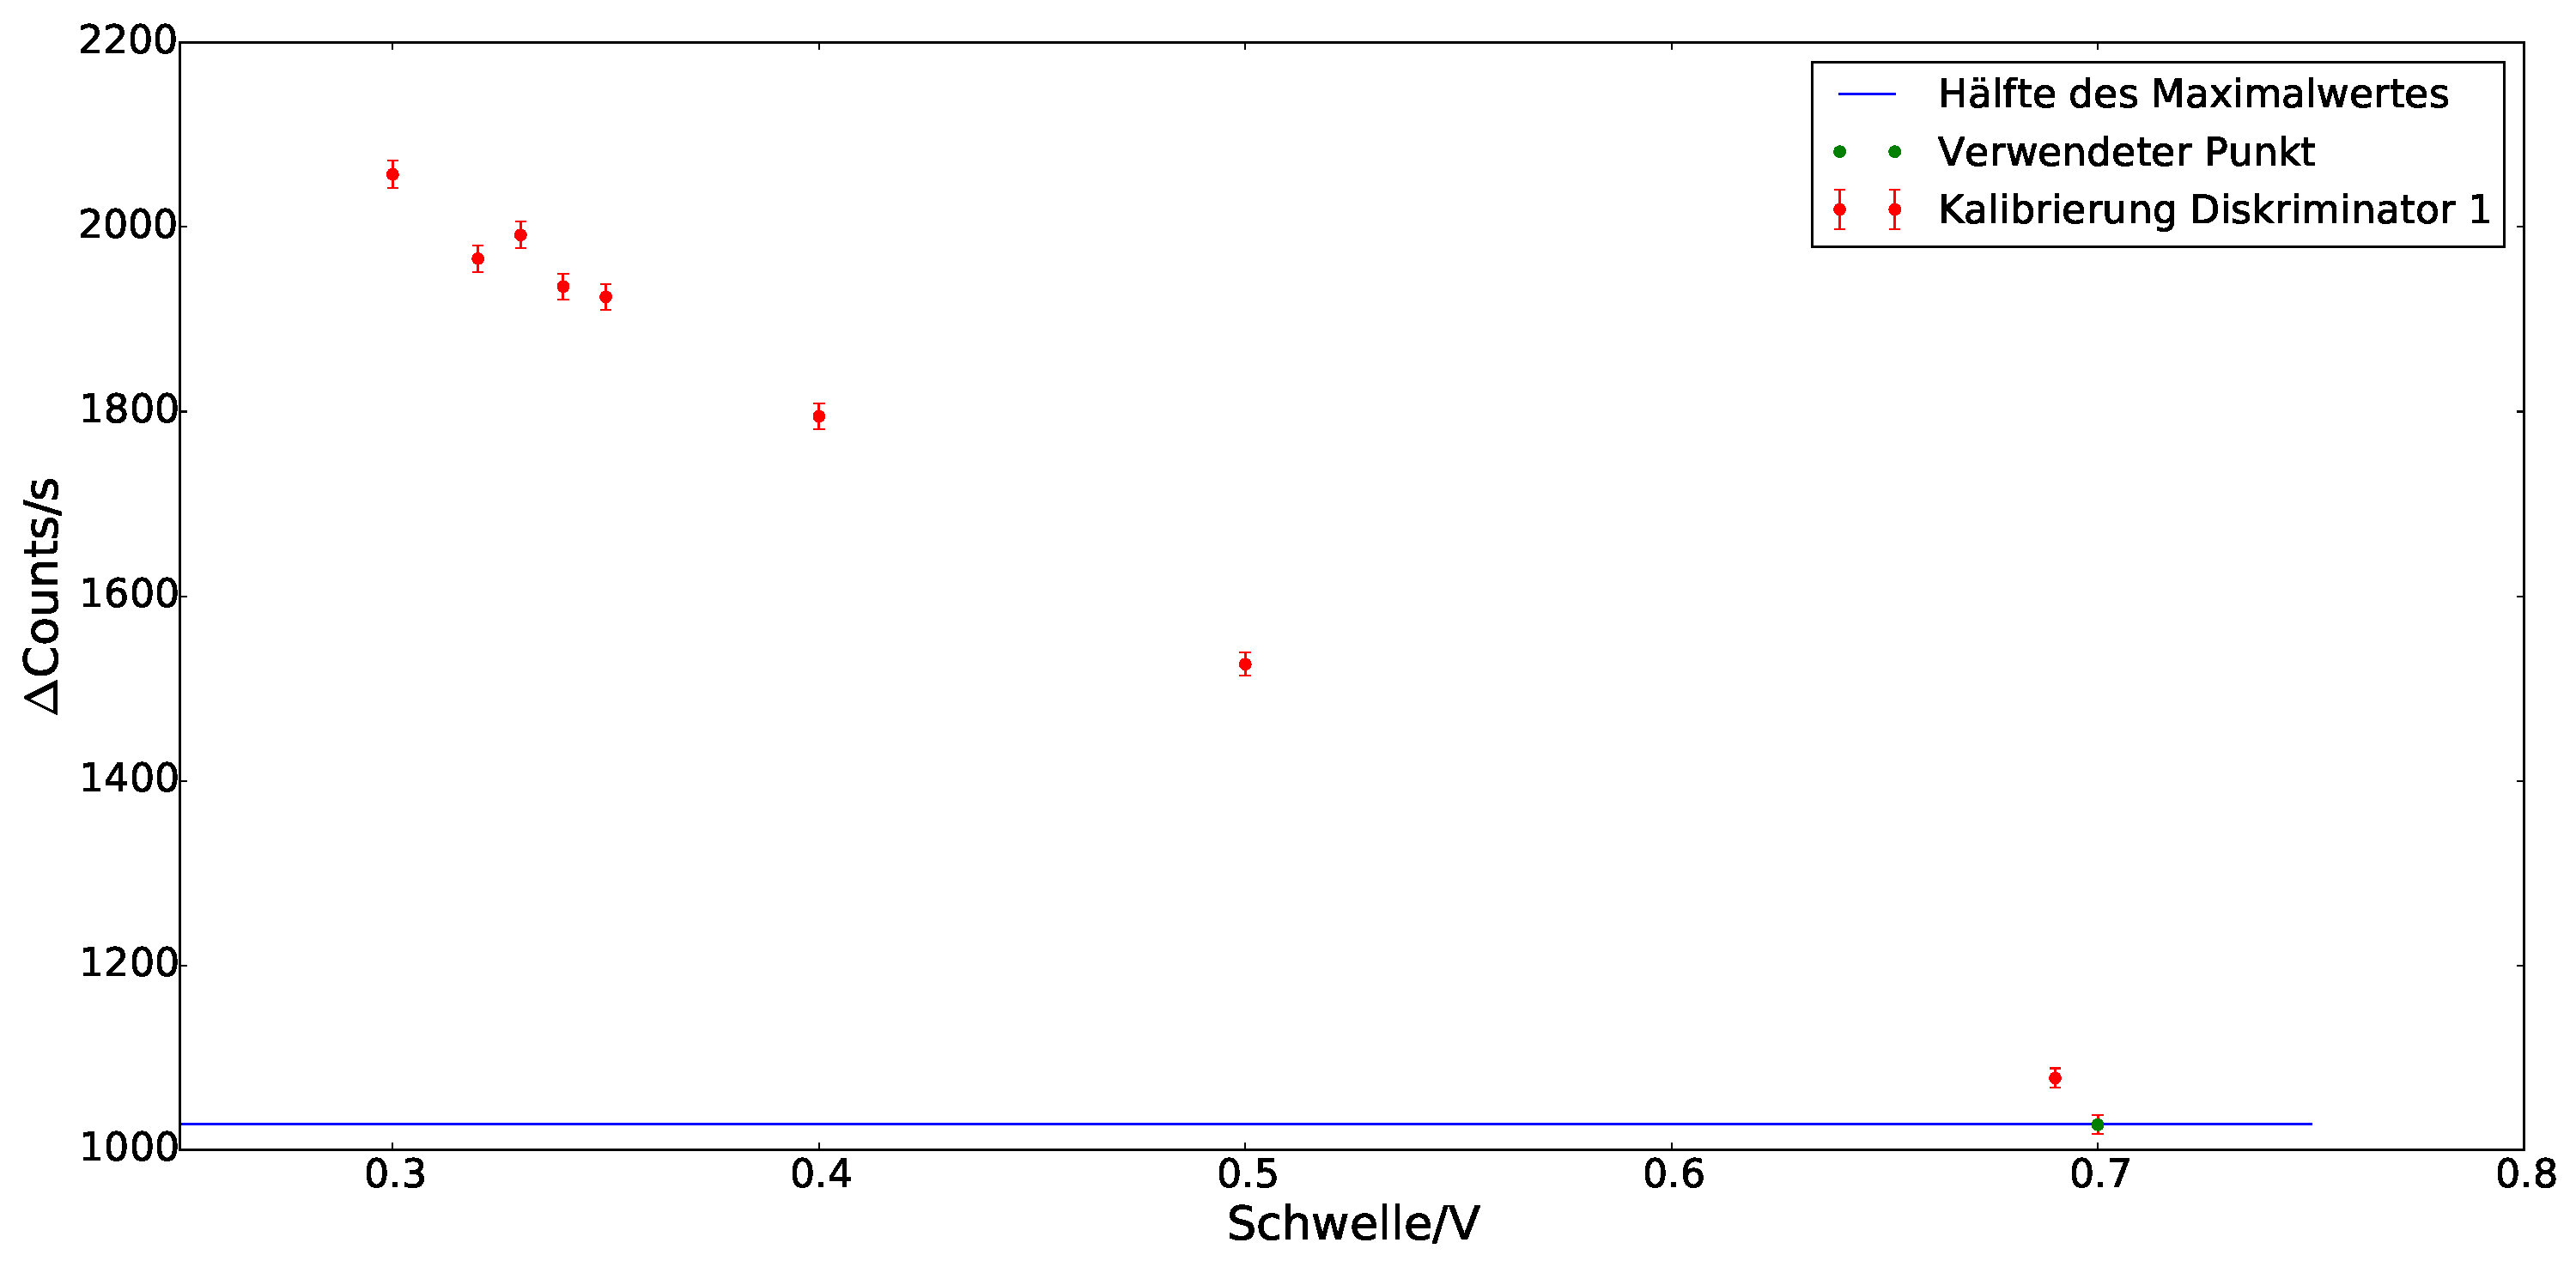
\includegraphics[scale = 0.35]{Disk_1.pdf}
\caption{Differenzplot der Counts gegen die Schwellspannung f�r Diskriminator 1}
\label{fig:Disk_1}
\end{figure}
\begin{figure}[H]
\centering
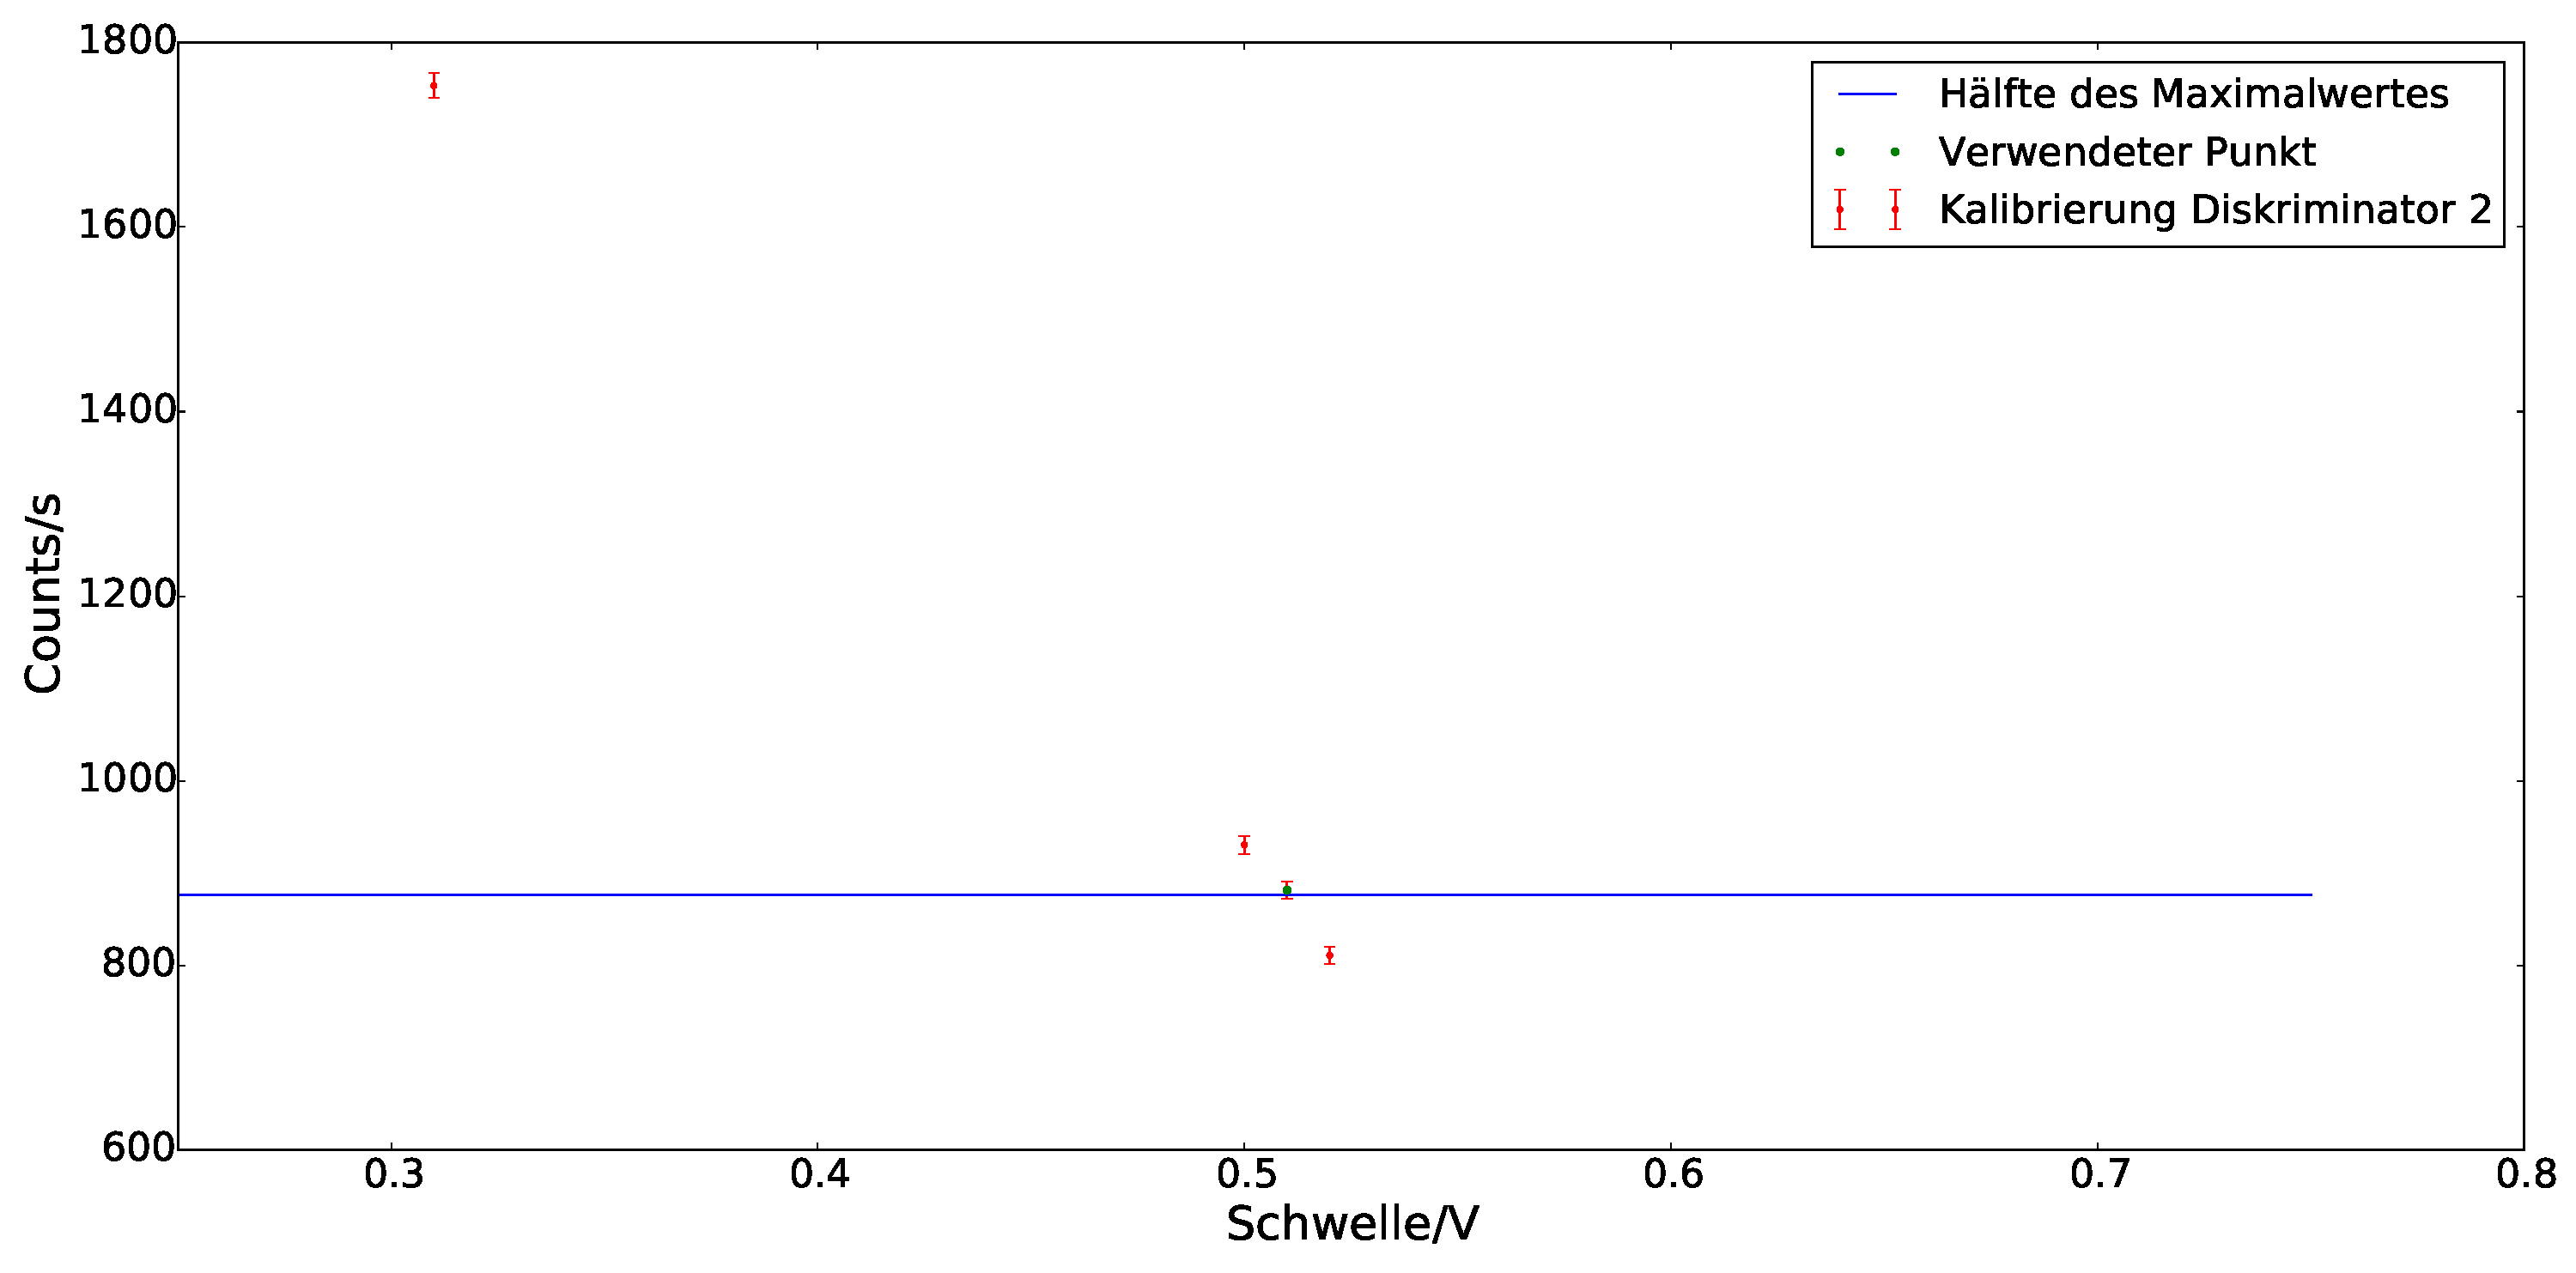
\includegraphics[scale = 0.35]{Disk_2.pdf}
\caption{Differenzplot der Counts gegen die Schwellspannung f�r Diskriminator 2}
\label{fig:Disk_2}
\end{figure}
In Abb. \ref{fig:Disk_3} wurde zus�tzlich eine etwas h�here Schwelle eingestellt, welche auf H�he des Plateaus zwischen den beiden Energien der von $^{60}$Co emittierten Photonen liegt. Nach der Einstellung des Delays, wodurch erreicht werden soll, dass die beiden oberen Szintillatoren (1 und 2) gleichzeitig mit dem 3. Szitillator triggern, wird die Diskriminatorschwelle f�r den 3. Szintillator auf den h�heren Wert gestellt, sodass dieser w�hrend der Messung nur bei Zerfall eines Myons triggert. Szintillator 1 und 2 triggern w�hrend der Messung genau beim Eintritt des Myons in Szintillator 3, wobei Szintillator 3 erst im Falle eines Zerfalls triggert (2. Diskriminatorschwelle). 
\begin{figure}[H]
\centering
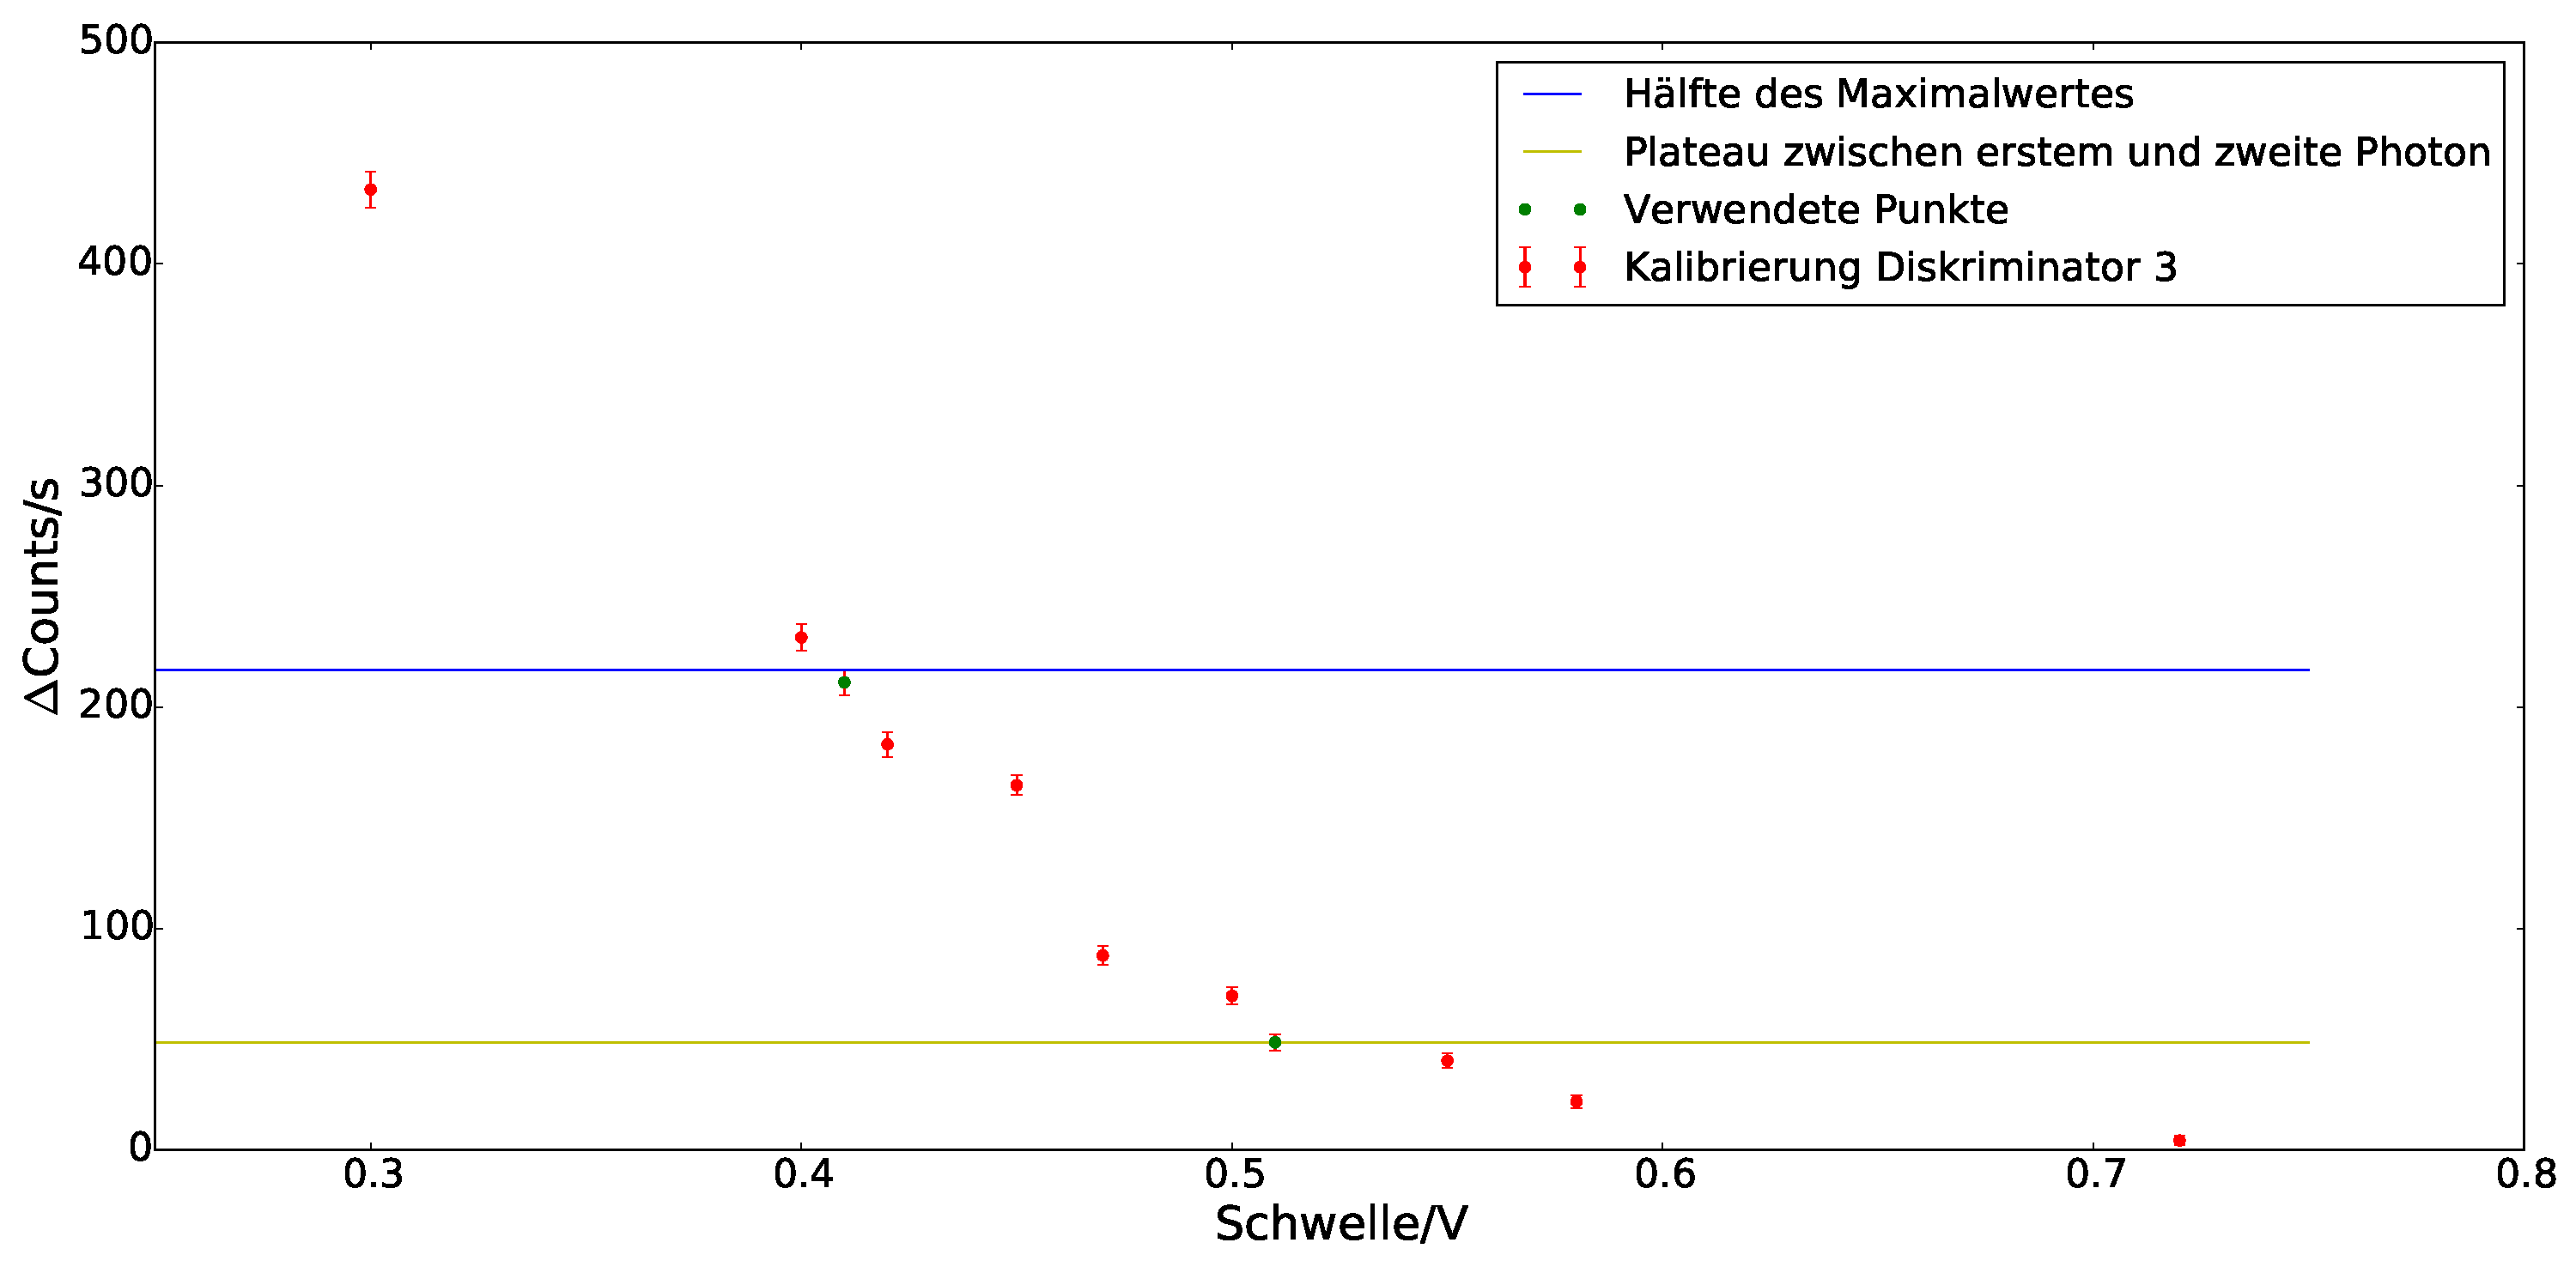
\includegraphics[scale = 0.35]{Disk_3.pdf}
\caption{Differenzplot der Counts gegen die Schwellspannung f�r Diskriminator 3}
\label{fig:Disk_3}
\end{figure}
\begin{figure}[H]
\centering
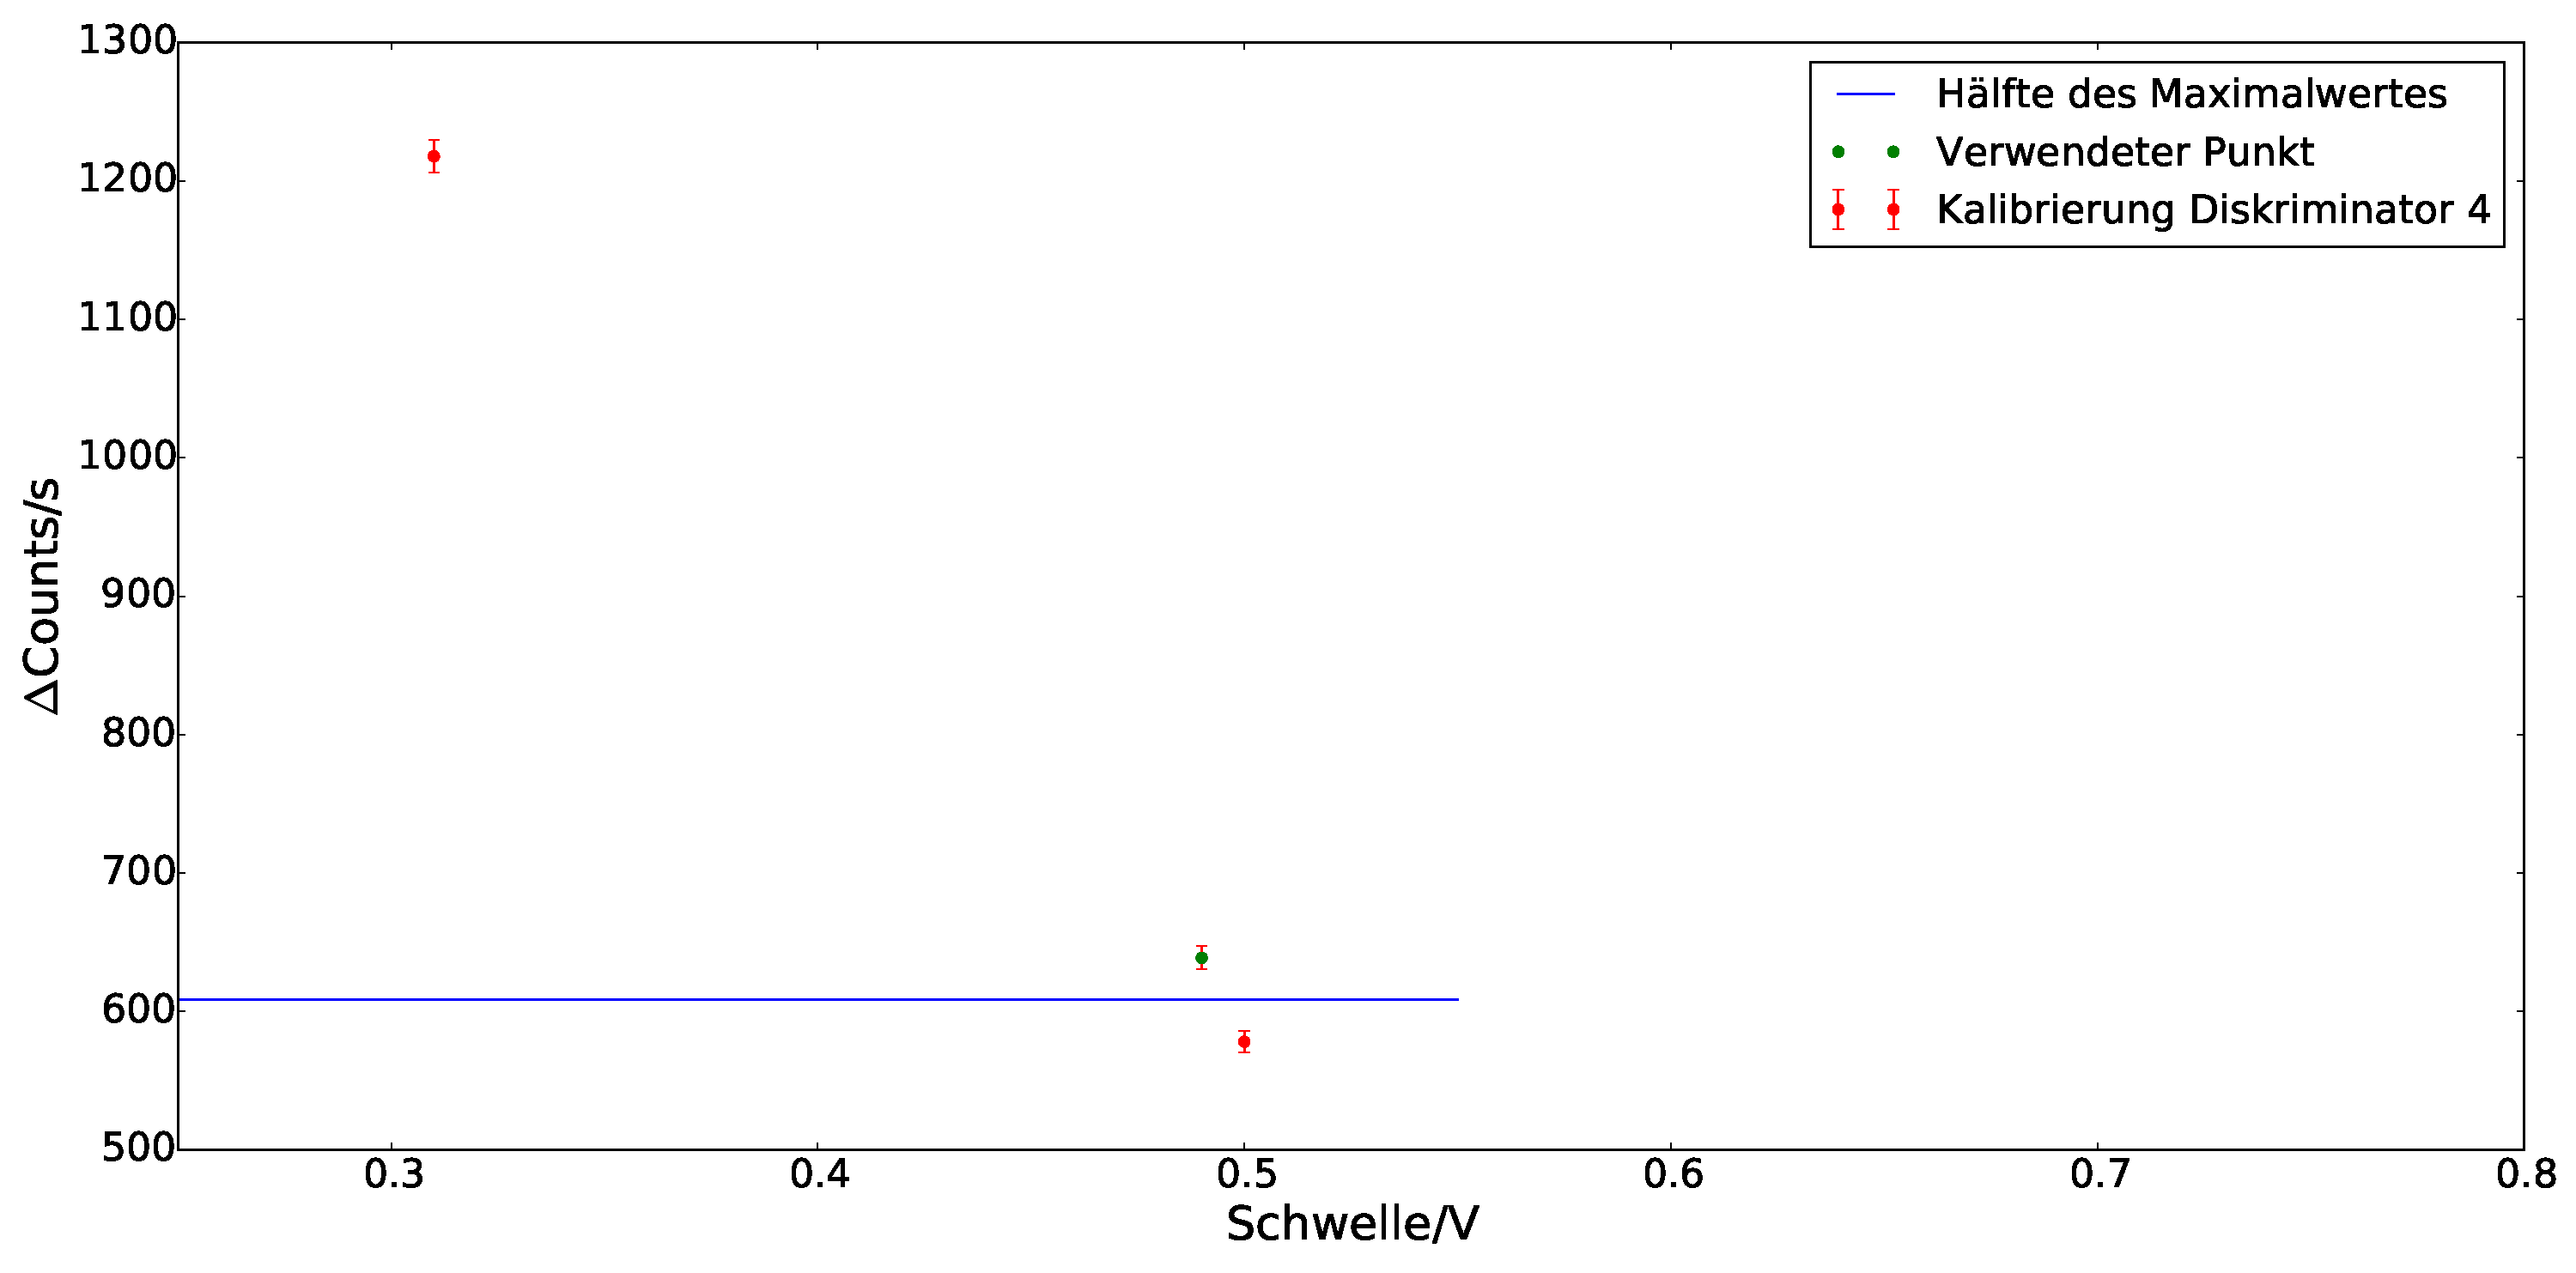
\includegraphics[scale = 0.35]{Disk_4.pdf}
\caption{Differenzplot der Counts gegen die Schwellspannung f�r Diskriminator 4}
\label{fig:Disk_4}
\end{figure}
Die Energien der Photonen beim Zerfall von $^{60}$Co werden in Abb. \ref{fig:Co_60} dargestellt.(vgl. \cite{Co_60})
\begin{figure}[H]
\centering
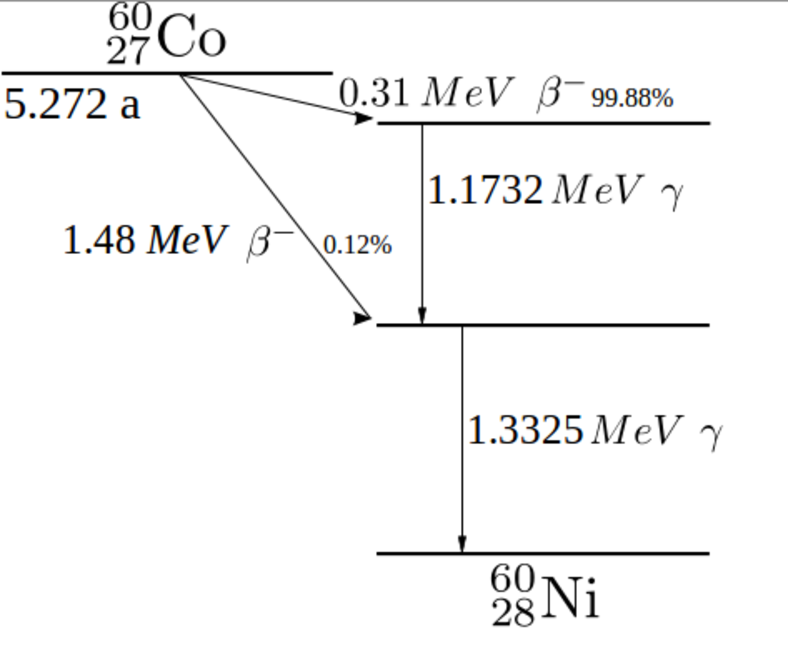
\includegraphics[trim = 0cm 0cm 0cm 1.1nm,scale = 0.5, clip]{Cobalt60_Zerfall.pdf}
\caption{Zerfall von $^{60}$Co}
\label{fig:Co_60}
\end{figure}
In Tabelle \ref{tab:Schwellwerte} sind die Diskriminatorschwellen f�r Diskriminator 1 bis 4 aufgelistet.
\begin{table}[H]
\caption{Diskriminatorschwellwerte}
\begin{tabular}{c|c|c|c|c|}
 & Diskriminator 1 & Diskriminator 2 & Diskriminator 3 & Diskriminator 4 \\ 
\hline Untere Schwelle & 0,70 V & 0,51 V & 0,41 V & 0,49 V \\ 
\hline Obere Schwelle &  &  & 0,52 V &  \\ 
\hline 
\end{tabular}
\label{tab:Schwellwerte}
\end{table}
\subsection{Delay}
Da PM1, PM2 und PM4 �ber eine logische Einheit verbunden sind, welche den TAC startet, muss sichergestellt werden, dass die Signale der drei Photomuliplier Zeitgleich ankommen. Die Zeitversetzung (Delay) der Signale wird �ber die Kabell�nge der Photomuliplier zur logischen Einheit eingestellt.

Es kann angenommen werden, das die Signale von PM3 und PM4 zur selben Zeit ankommen. Deshalb kann das Signal von PM3 gut als Referenz f�r die ersten beiden verwendet werden. F�r die Bestimmung des Delays werden PM1 (bzw. PM2) und PM3 an die logische Einheit angeschlossen, jedoch ohne ein Veto. Die Szintillatoren werden so geschaltet, dass nur bei gleichzeitigem Signal hochgez�hlt wird. Es wird erwartet, das sich ein Plateau ausbildet. Der Delay in der Mitte des Plateaus ist die optimale Einstellung, das sich die Signale an diesem Punkt �berlagern. Damit sich ein m�glichst schmales Plateau ausbildet, m�ssen die Pulse der Diskriminatoren kurz sein. In Abbildung \ref{fig:delay_1} ist zu sehen, dass f�r den ersten Photomulipier kein eindeutiges Plateau identifiziert werden konnte. Deshalb musste das Delay mit dem Oszilloskop eingestellt werden, um sicherzustellen, dass sich die beiden Signale �berlappen. F�r den ersten Photomuliplier wurde mit dem Oszilloskop ein Delay von 9ns bestimmt. In Abbildung \ref{fig:delay_2} sind die Messdaten f�r den zweiten Photomuliplier zu sehen. Im Bereich von 20 bis 28ns ist ein Plateau zu erkennen, das Delay wurde mit dem Wert (24ns) in der Mitte des Plateaus angenommen. Das Delay von 24ns f�r den zweiten Photomuliplier wurde zus�tzlich mit dem Oszilloskop bestimmt und konnte best�tigt werden.

\begin{figure}[H]
	\centering
  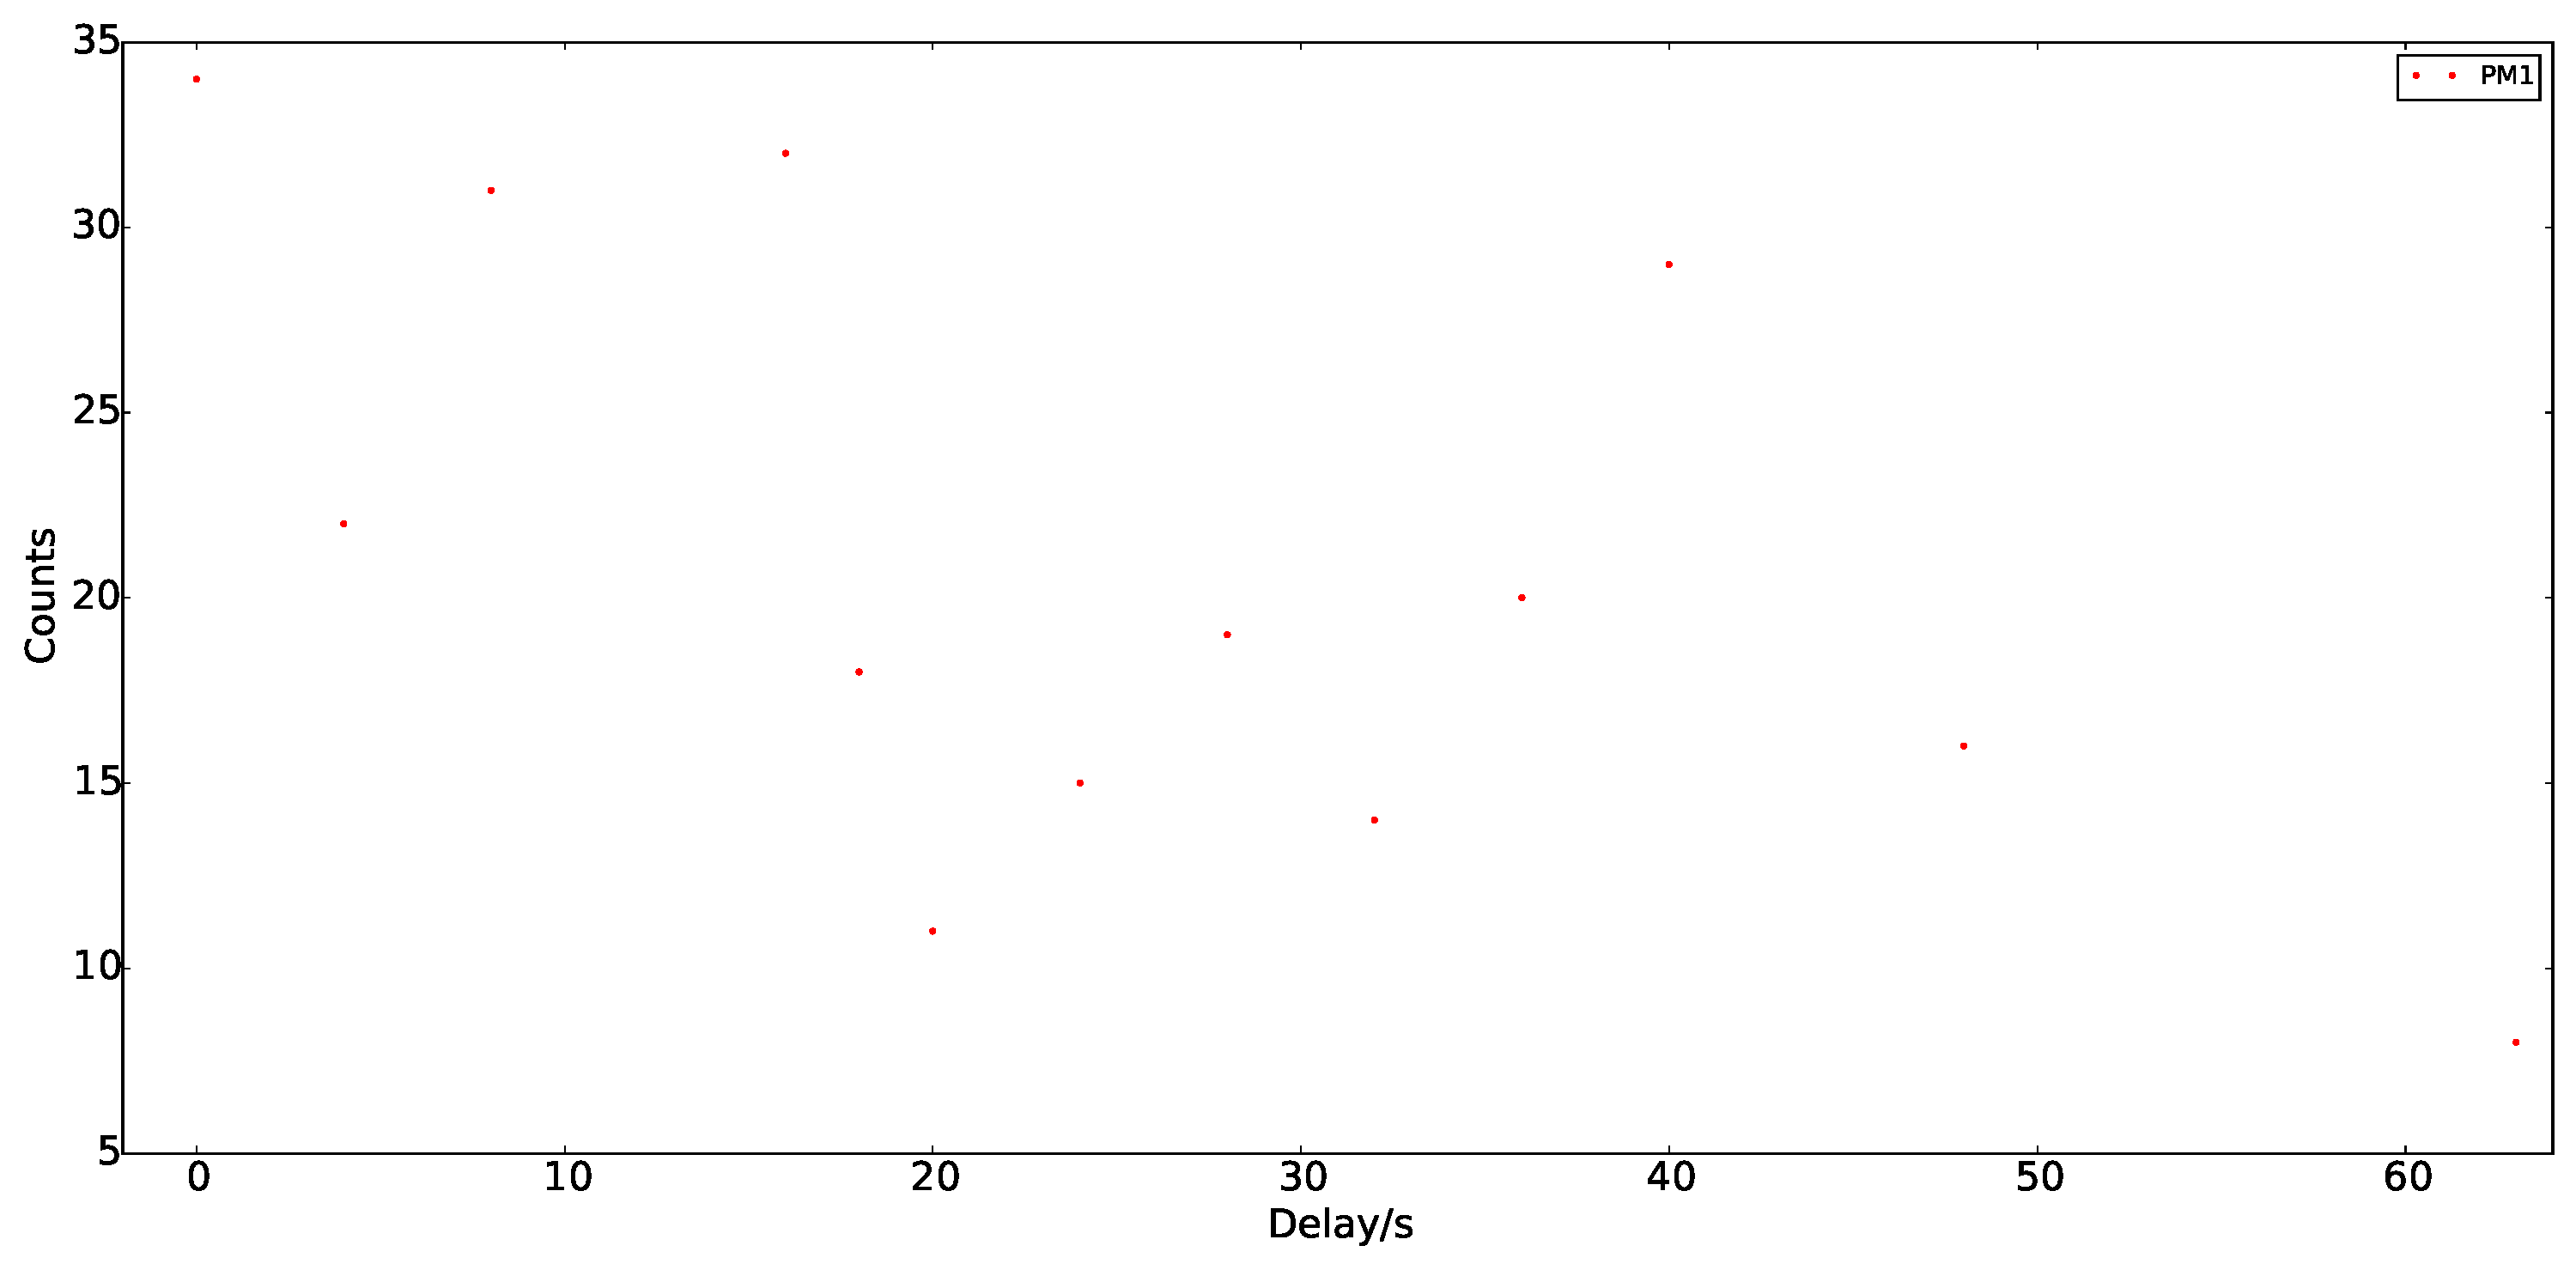
\includegraphics[scale=0.33]{delay_1.pdf}
	\caption{Counts in Abh�ngigkeit vom Delay f�r die ersten Photomuliplier, es ist kein eindeutiges Plateau zu erkennen. Deshalb wurde das Signal mit einem Oszilloskop betrachtet und ein Delay von 9ns bestimmt.}
	\label{fig:delay_1}
\end{figure}


\begin{figure}[H]
	\centering
  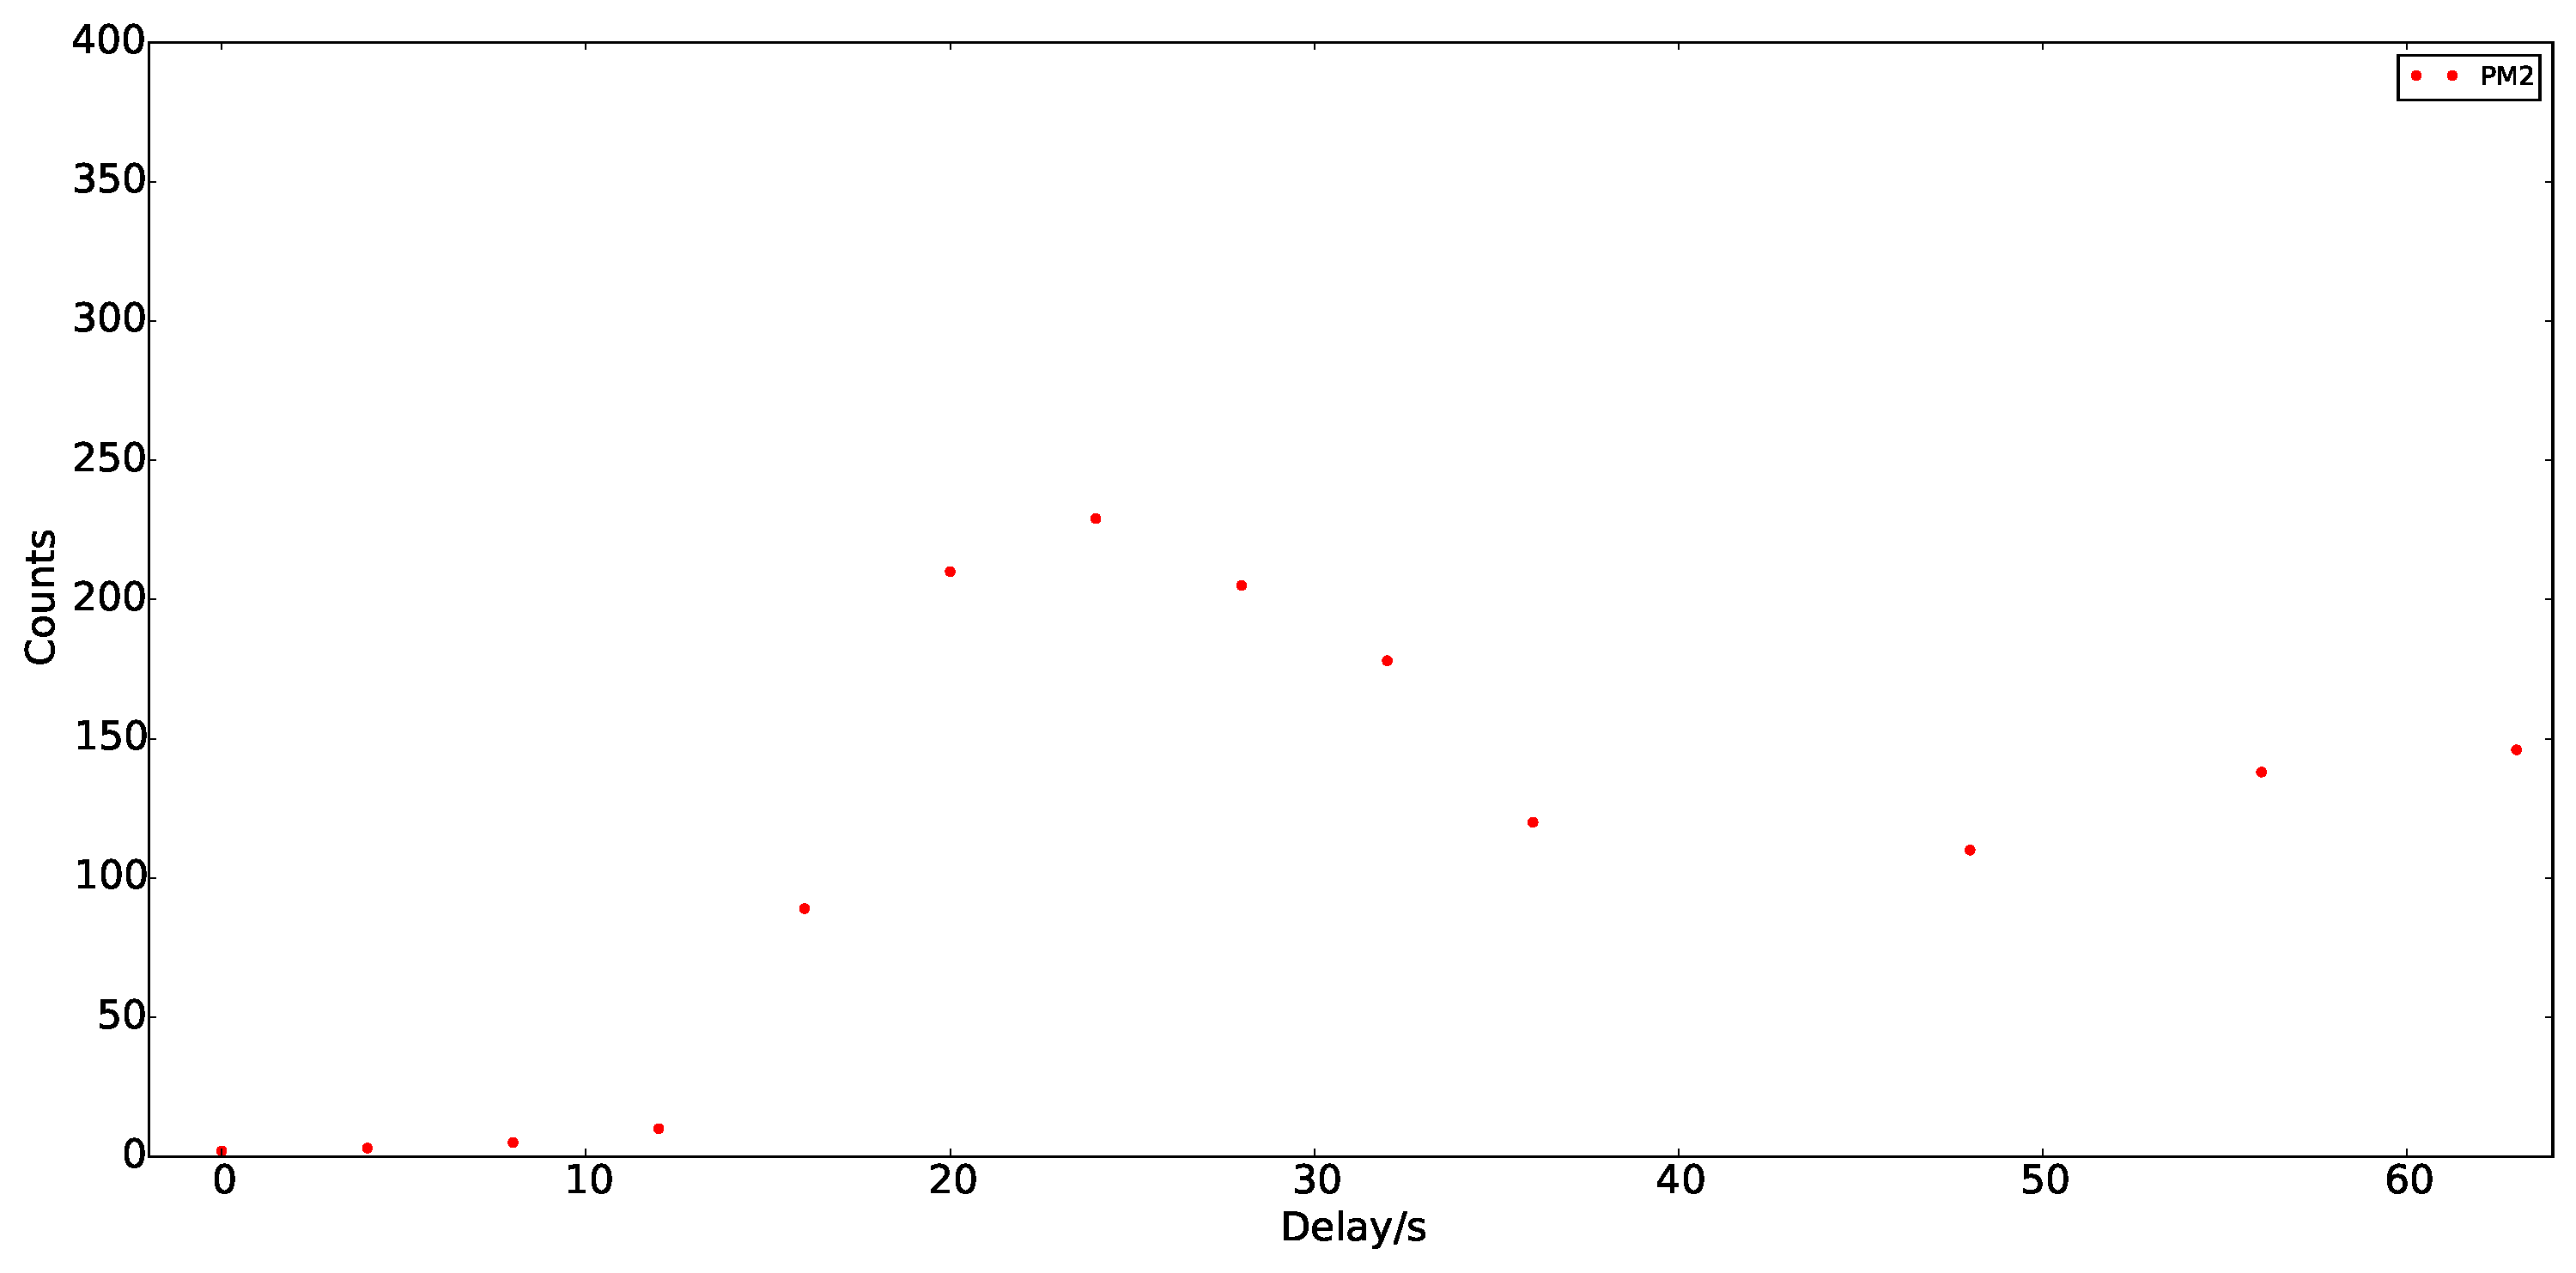
\includegraphics[scale=0.33]{delay_2.pdf}
		\caption{Counts in Abh�ngigkeit vom Delay f�r die ersten Photomuliplier. Ein Plateau ist im Bereich von 20 bis 28 ns zu erkennen. Das Delay wurde mit 24 ns, in der Mitte des Plateaus bestimmt. dieser Wert wurde mit dem Oszilloskop verifiziert.}
	\label{fig:delay_2}
\end{figure}

Es ergeben sich die Delays in Tabelle \ref{tab:delay}.

\begin{table}[H]
	\centering
	\caption{Optimal bestimmtes Delay f�r PM1 und PM2}
	\label{tab:delay}
	\begin{tabular}{|c|c|}
	\hline Photomuliplier & Delay [ns] \\ \hline
	\hline PM1 & 9 \\ 
	\hline PM2 & 24 \\ 
	\hline 
	\end{tabular} 
\end{table}

Das Oszilloskopbild Abb. \ref{PMT2Delay} zeigt, dass die Signale beim zweiten Photomultiplier �bereinander liegen. Auff�llig war, dass trotz Abschlusswiderstand verschobene Signale angezeigt wurden, die eigentlich nicht zu sehen sein sollten.
\begin{figure}[H]
\centering
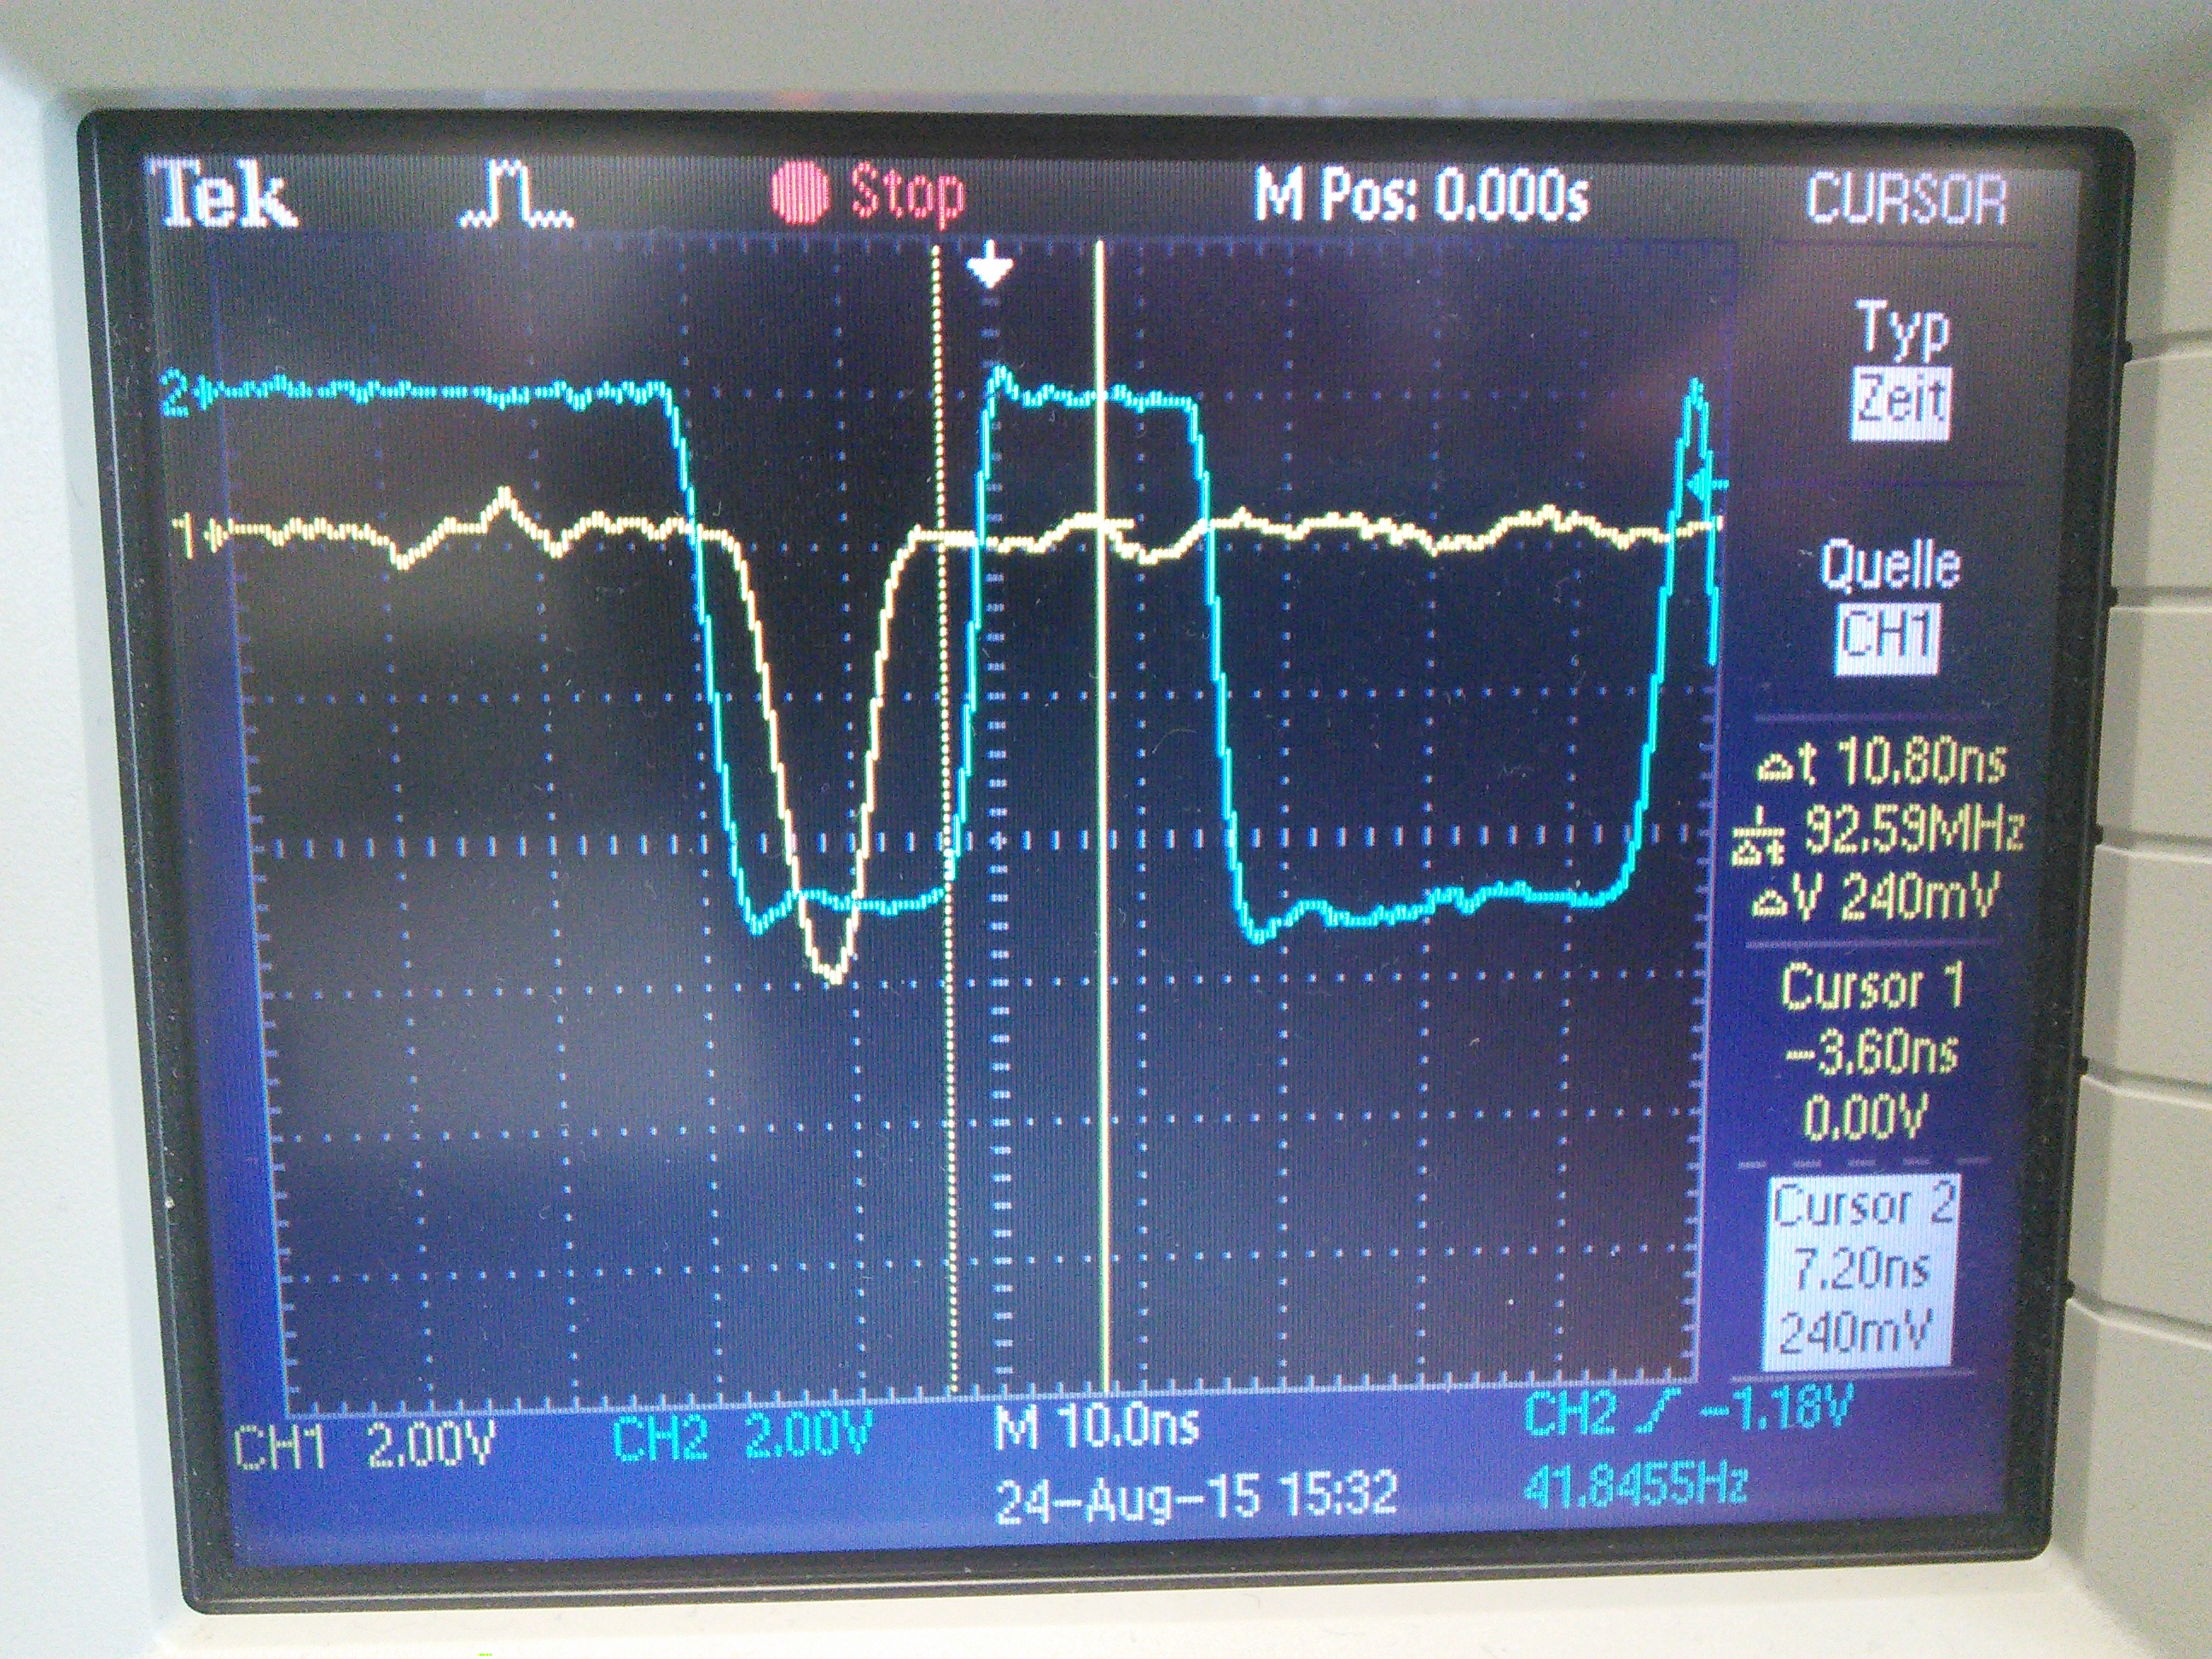
\includegraphics[scale=0.12]{DelayPMT2}
\caption{Oszilloskopbild Delay PMT 2}
\label{PMT2Delay}
\end{figure}
\subsection{Kanal-Zeit-Eichung}
F�r eine genaue Bestimmung der Lebensdauer von Myonen ist eine exakte Zeiteichung extrem wichtig. F�r die Zeiteichung wird ein TAC, ein dual Timer und ein Oszilloskop verwendet. Der schematische Aufbau ist in Abbildung \ref{fig:kanal_zeit} zu sehen. 

\begin{figure}[H] 
	\centering
  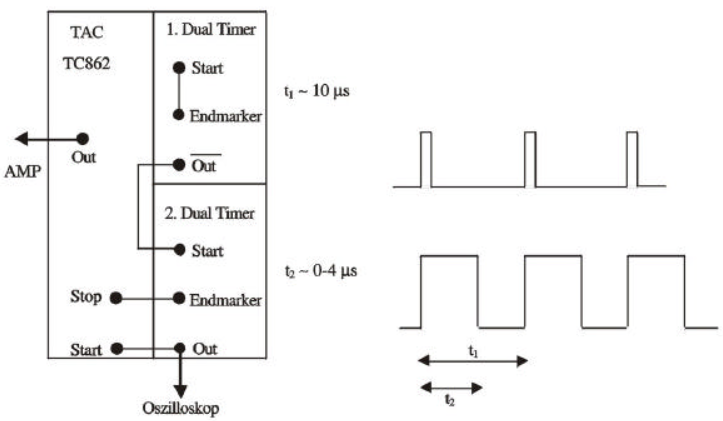
\includegraphics[scale=0.5]{kanal_zeit.png} 
	\caption{Schematischer Aufbau f�r die Kanal-Zeit-Eichung}
	\label{fig:kanal_zeit}
\end{figure}

Der dual Timer wird verwendet, um kurze Signale mit bekannter L�nge zu erzeugen. �ber die High und Lows des Signals wird der TAC gesteuert, wodurch eine Spannung in Abh�ngigkeit der L�nge des Signals erzeugt wird. Das Signal wird verst�rkt und mit dem ADC digitalisiert, damit es vom Mulit-Channel-Analyser verwertet werden kann. Durch variiren der Signall�nge lassen sich die verschiedene Kan�le ansprechen, wodurch eine Beziehung zwischen einer Zeit und einem Kanal hergestellt wird. Die Zeitintervalle werden gegen die Kan�le aufgetragen und mit Gleichung \ref{eqn:kanal} gefittet. Zum Vergleich soll zus�tzlich ein Fit mit $B = 0$ erzwungen werden. Die Parameter und Variablen des Fits sind in Tabelle \ref{tab:fit_kanal} zu sehen

\begin{align}
\label{eqn:kanal}
t = A*k+B
\end{align}

\begin{table}[H]
	\caption{Parameter des Fits}
	\label{tab:fit_kanal}
	\begin{tabular}{c|l}
	t & Zeitintervall in $\mu$s \\ 
	k & Kanal \\ 
	A & Proportionalit�tsfaktor \\ 
	B & Offset \\ 
	\end{tabular} 
\end{table}

In Abbildung \ref{fig:kanal_zeit_fit} sind die Messwerte zu sehen. F�r die Fitparameter ergaben sich dabei die Werte in Tabelle \ref{tab:fit}. Das $\chi_{red}^2$ hat ein Wert von 0,02, was einem guten Fit entspricht.

\begin{table}[H]
\centering
\caption{Fitparameter mit Fehlern und $\chi_{red}^2$}
\label{tab:fit}
\begin{tabular}{|c|c|}
\hline Paramter & Wert \\ 
\hline A & 0,002106(6) \\ 
\hline B & 0,126(19) \\ 
\hline $\chi_{red}^2$ & 0,233 \\ 
\hline 
\end{tabular} 
\end{table}

\begin{figure}[H] 
	\centering
	  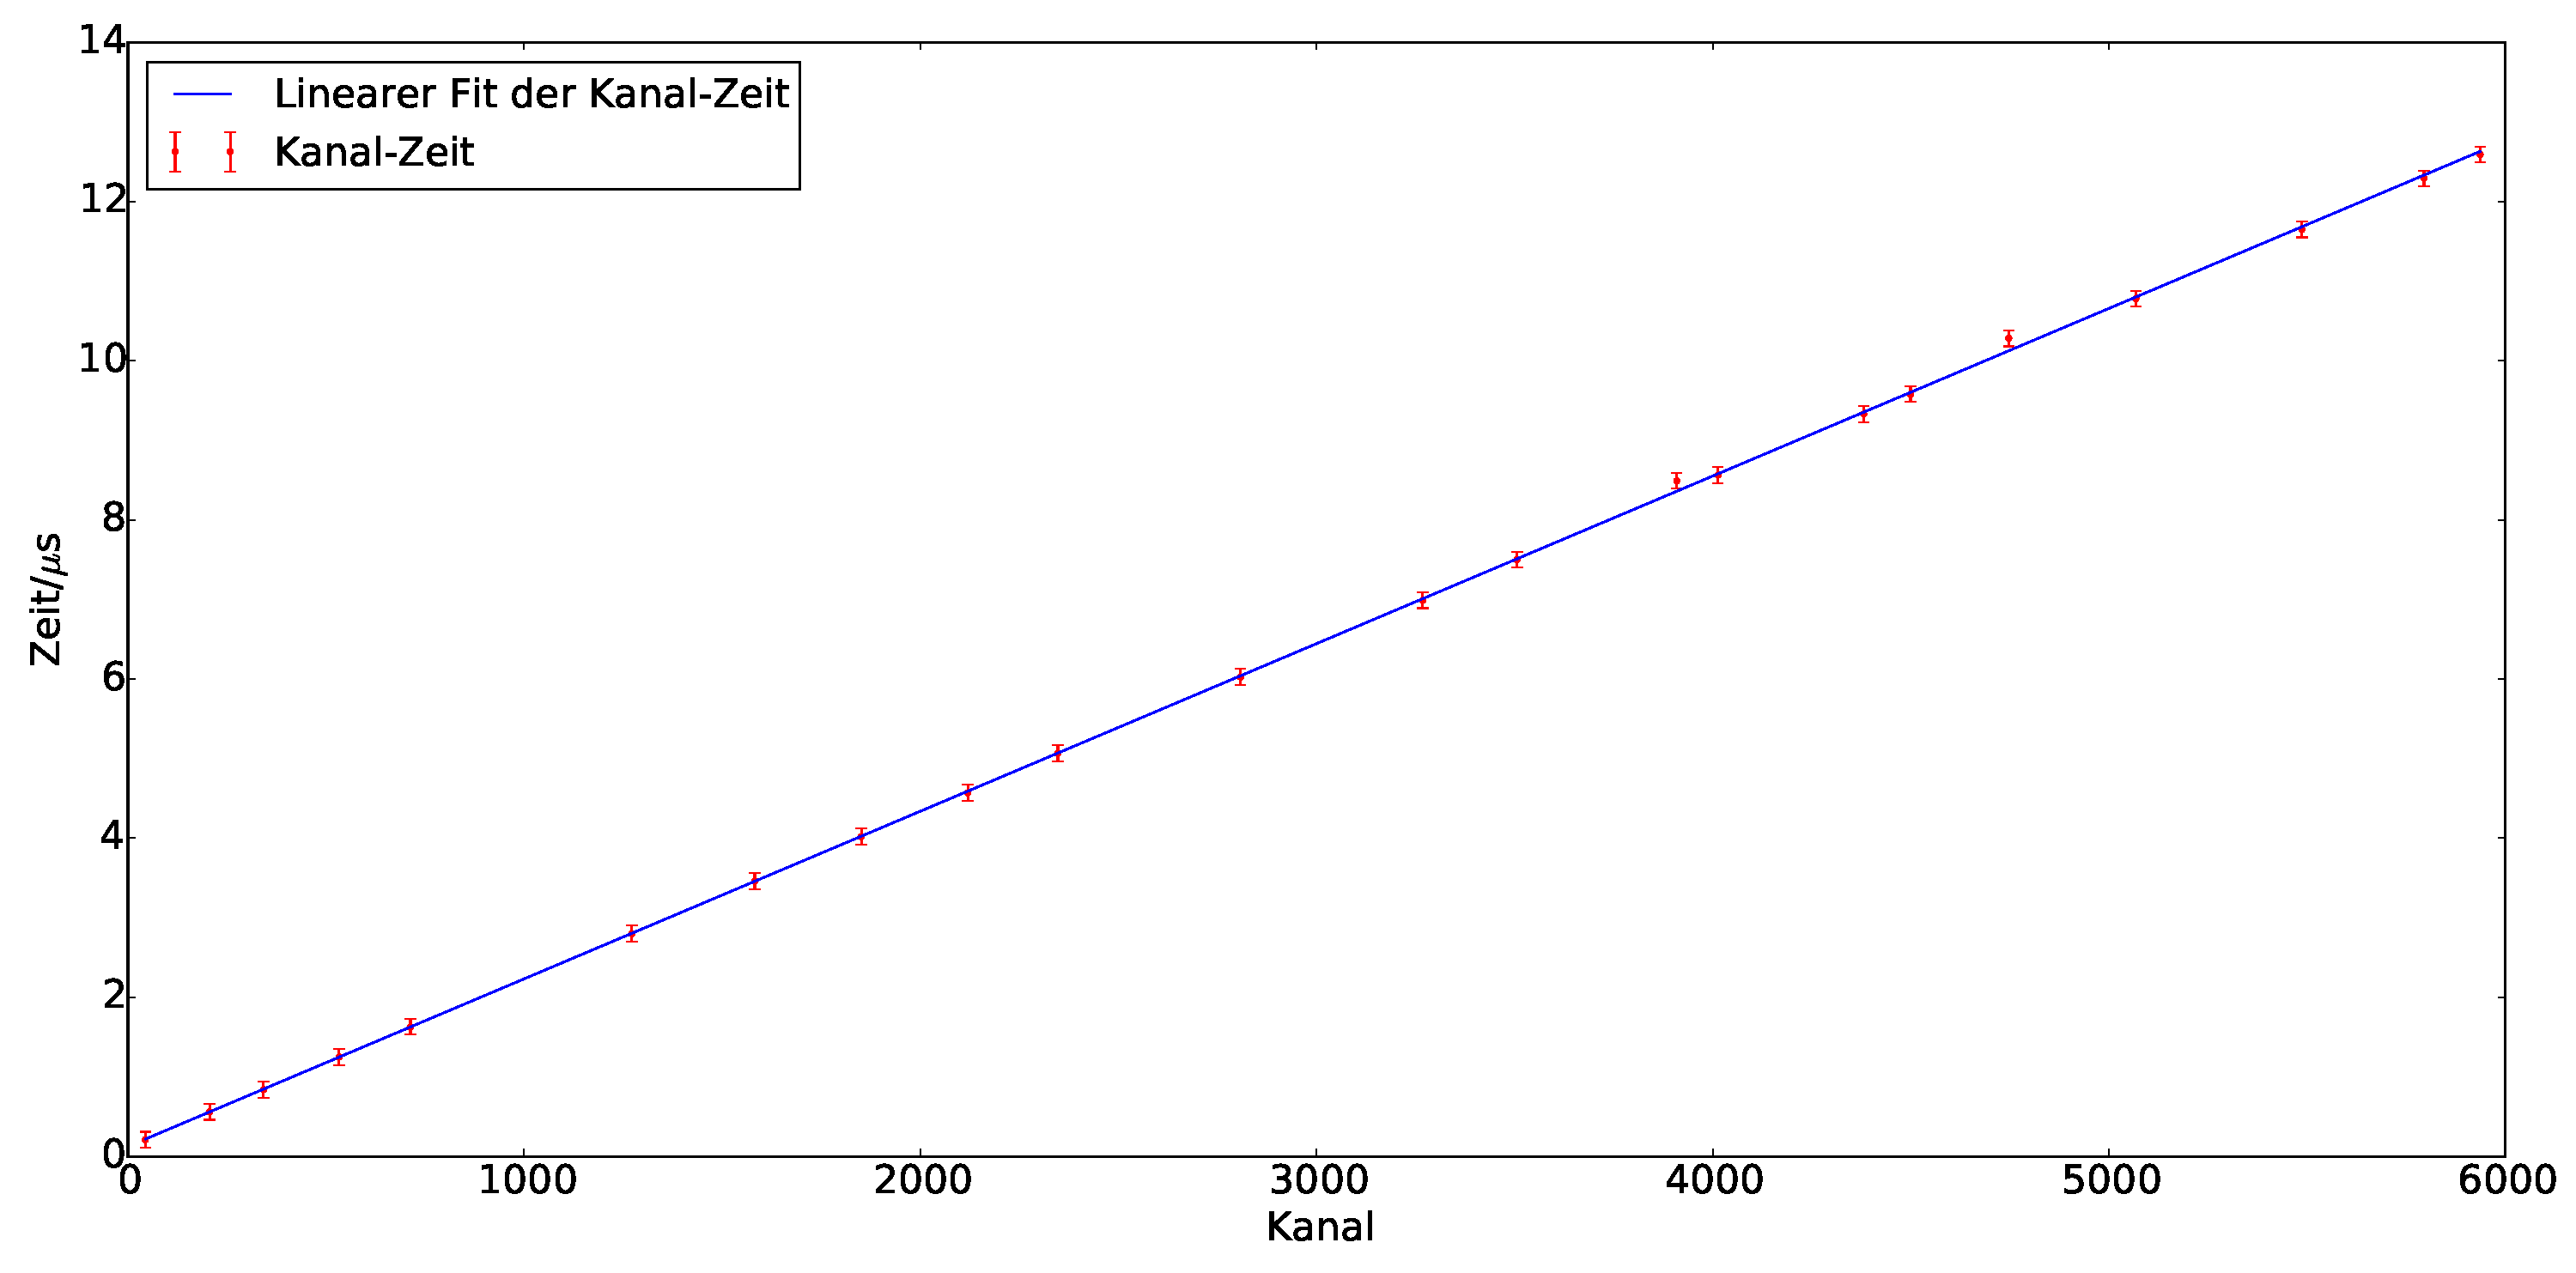
\includegraphics[scale=0.33]{kanal_zeitax+b.pdf} 
	\caption{Kanal-Zeit-Eichung}
	\label{fig:kanal_zeit_fit}
\end{figure}
Zum Vergleich sind die Fitparameter f�r $B = 0$ in Tabelle \ref{tab:fit2} zu sehen. Der Fit f�r $B = 0$ ist in Abb. \ref{fig:kanal_zeit_fit2} dargestellt.
\begin{table}[H]
\centering
\caption{Fitparameter mit Fehlern und $\chi_{red}^2$ f�r $B = 0$}
\label{tab:fit2}
\begin{tabular}{|c|c|}
\hline Paramter & Wert \\ 
\hline A & 0.002136(5) \\ 
\hline B & 0 \\ 
\hline $\chi_{red}^2$ & 0,719 \\ 
\hline 
\end{tabular} 
\end{table}
\begin{figure}[H] 
	\centering
	  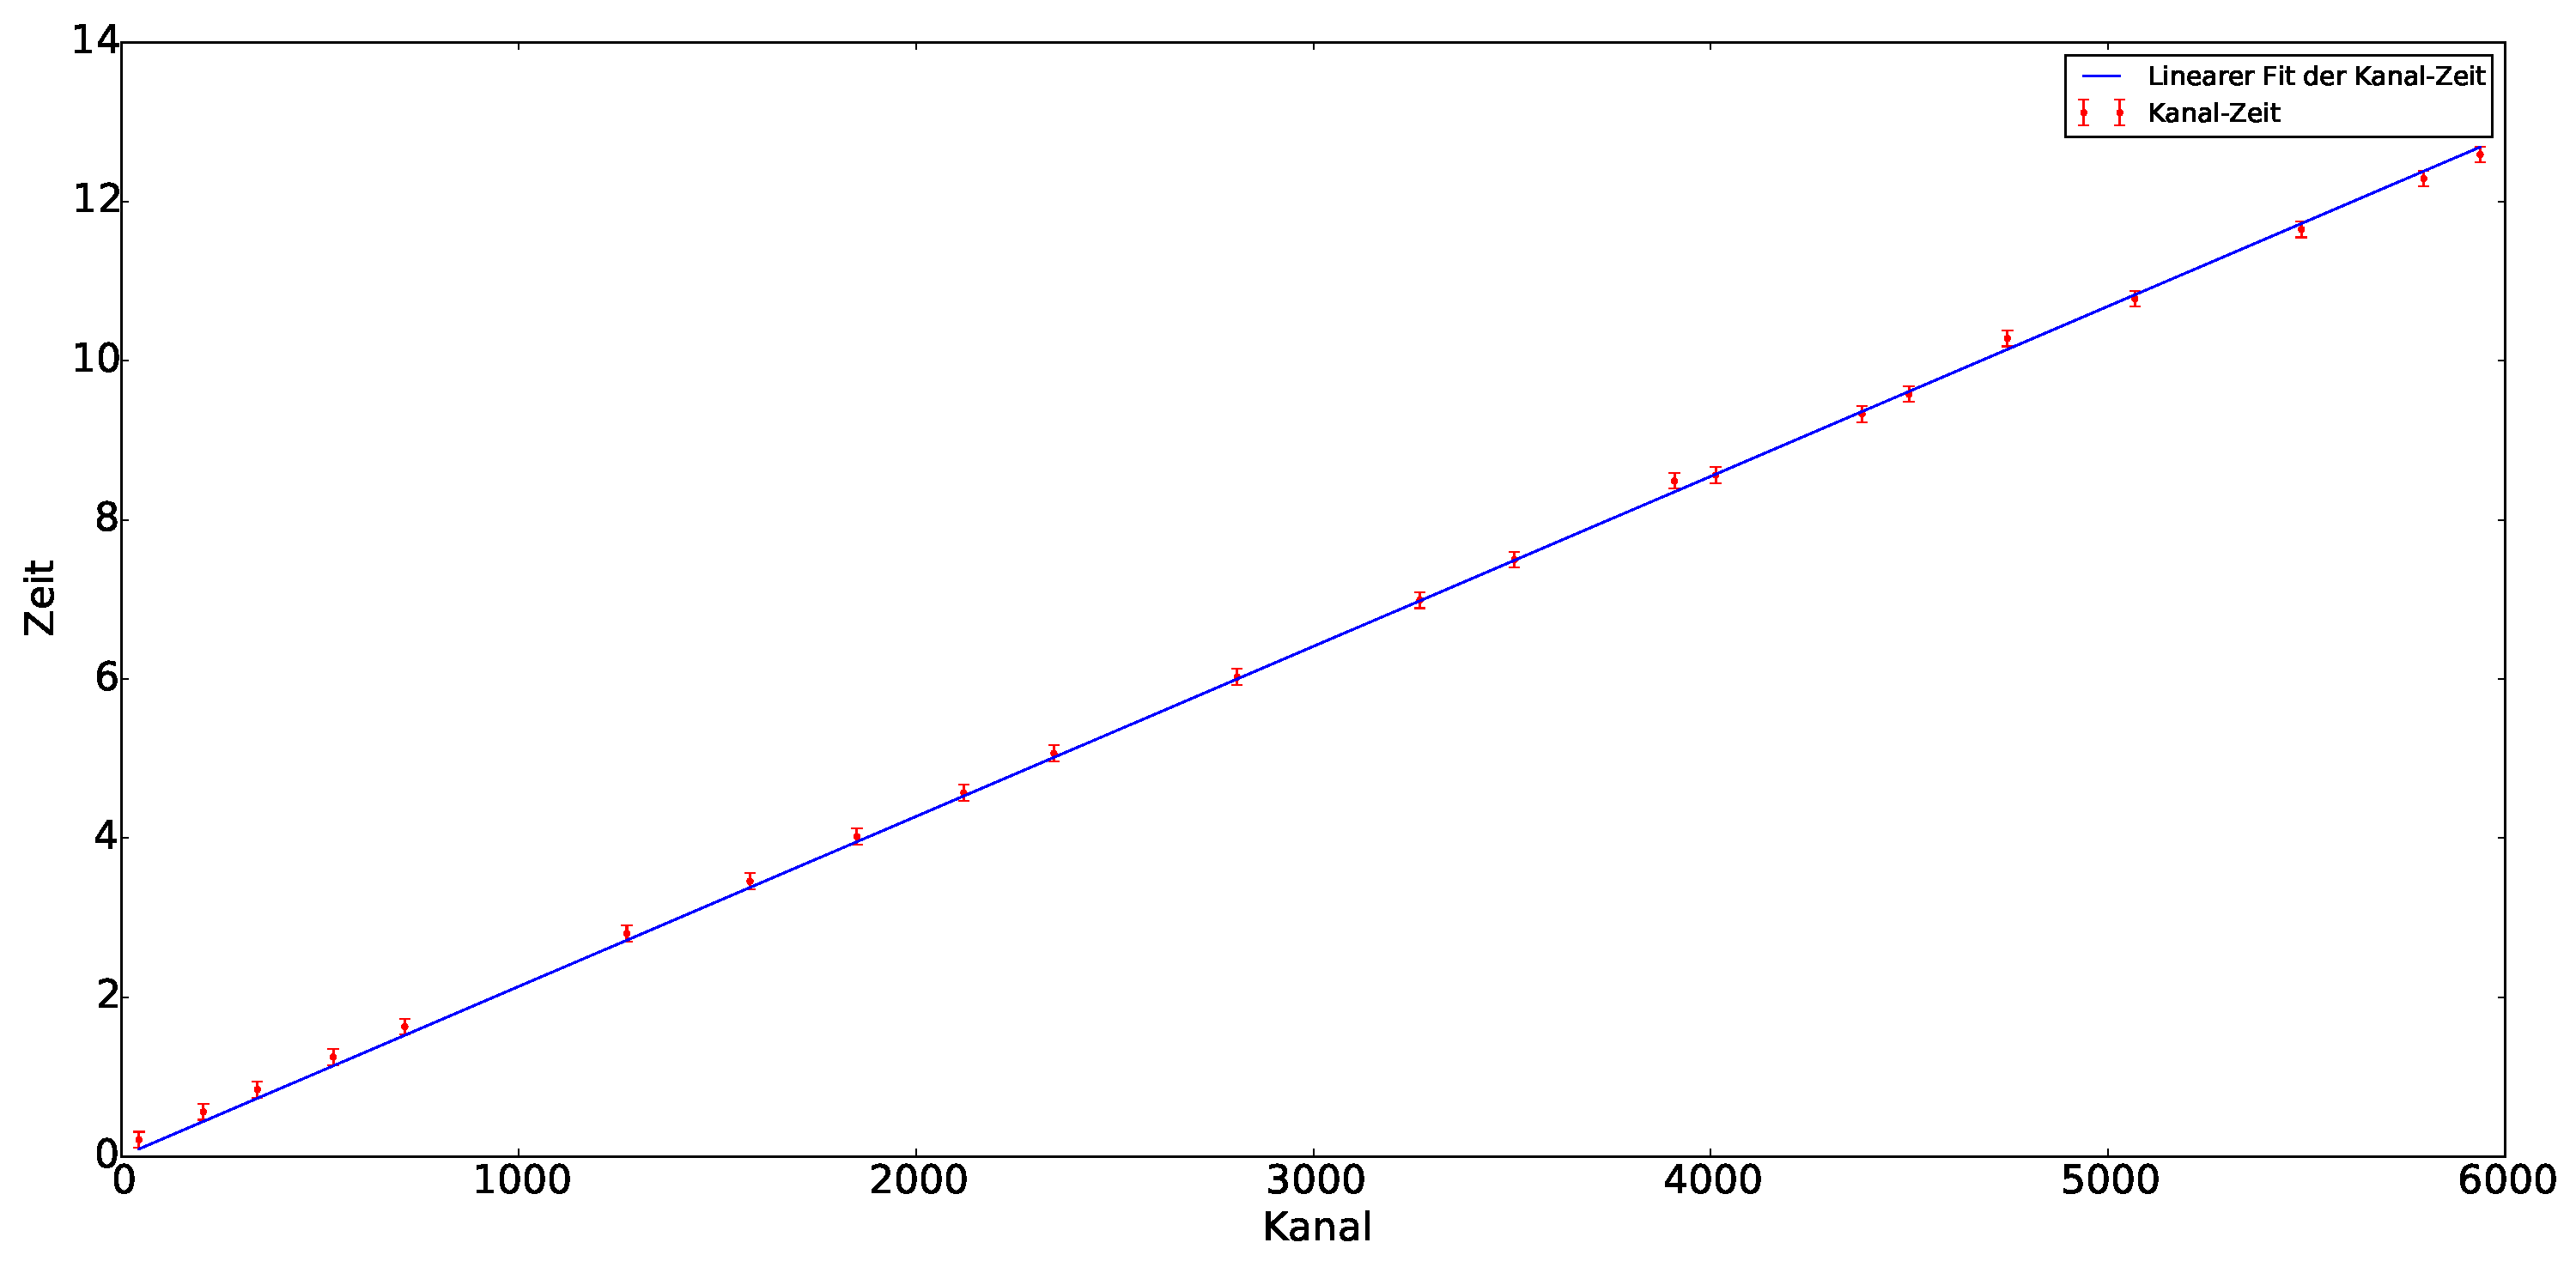
\includegraphics[scale=0.33]{kanal_zeitax.pdf} 
	\caption{Kanal-Zeit-Eichung f�r $B = 0$}
	\label{fig:kanal_zeit_fit2}
\end{figure}
\subsection{Messung der mittleren Lebensdauer}
Nachdem die umfangreichen Kalibrationen beendet sind, soll die Lebensdauer der Myonen anhand der Messdaten bestimmt werden. Dazu werden die folgenden Methoden verwendet und deren Resultat verglichen.
\subsubsection{Maximum Likelihood Methode}
Um die mittlere Lebensdauer von Myonen zu bestimmen eignet sich die Maximum Likelihood Methode. Wie in Abschnitt 2.3 besprochen sind Zerfallszeiten mit Zeitunabh�ngiger Zerfallsrate exponentialverteilt, sodass sich die einparametrige Warscheinlichkeitsdichte
\begin{align}
P(t_i|\tau) = \frac{1}{\tau}\frac{e^{-\frac{t_i}{\tau}}}{e^{-\frac{T_1}{\tau}}-e^{-\frac{T_2}{\tau}}}
\end{align}
ergibt. Da die Messung des Zeitintervalls nach oben und unten beschr�nkt ist, wurde die Warschenlichkeitsdichte normiert, wobei $T_1$ die untere Schranke und $T_2$ die obere Schranke der Zeitmessung ist. Es wird davon ausgegangen, dass die einzelnen Zeitmessungen unabh�ngig voneinander sind, sodass sich f�r die gesamte Messung die n-dimensionale Warscheinlichkeitsdichte
\begin{align}
L = \prod_{i=1}^N P(t_i|\tau) = \prod_{i=1}^N \frac{1}{\tau}\frac{e^{-\frac{t_i}{\tau}}}{e^{-\frac{T_1}{\tau}}-e^{-\frac{T_2}{\tau}}}
\end{align}
ergibt. Es wird davon ausgegangen, dass die gemessenen Zerfallszeiten der wahrscheinlichsten Messung entsprechen, sodass die Messung einem Maximum der Warscheinlichkeitsdichtefunktion bez�glich $\tau$ entspricht. Um das Maximum von $L$ zu bestimmen betrachtet man die Funktion
\begin{align}
\ln{L} = \ln\left[\prod_{i=1}^N P(t_i|\tau)\right] = \sum_{i=1}^{N}\ln[P(t_i|\tau)] = -\left[\sum_{i=1}^{N}\ln(\tau) + \frac{t_i}{\tau} + \ln(e^{-\frac{T_1}{\tau}}-e^{-\frac{T_2}{\tau}})\right]
\end{align}
und bestimmt die Nullstelle der Ableitung nach $\tau$.
Schlie�lich erh�lt man die beste Approximation f�r die Lebensdauer $\tau$:
\begin{align}
\hat{\tau} = \frac{1}{N}\sum_{i=1}^{N} t_i - \frac{T_1e^{-\frac{T_1}{\tau}}-T_2e^{-\frac{T_2}{\tau}}}{e^{-\frac{T_1}{\tau}}-e^{-\frac{T_2}{\tau}}}
\end{align}
Da es nur M Kan�le und damit M m�gliche Zeiten $t_k$ gibt, kann die erste Summe umgeschrieben werden,
\begin{align}
\sum_{i=1}^{N} t_i = \sum_{k=1}^{M} N_k t_k \text{ wobei } N = \sum_{k=1}^{M} N_k
\end{align}
sodass der Fehler von $\hat{\tau}$ �ber den statistischen Fehler auf $N_k$, welcher $\sqrt{N_k}$ betr�gt, bestimmt werden kann.
Es ergibt sich also
\begin{align}
\hat{\tau} = \sum_{k=1}^{M} N_k t_k - \frac{T_1e^{-\frac{T_1}{\tau}}-T_2e^{-\frac{T_2}{\tau}}}{e^{-\frac{T_1}{\tau}}-e^{-\frac{T_2}{\tau}}}
\end{align}
mit einem Fehler von
\begin{align}
\Delta\hat{\tau} = \frac{1}{N}\sqrt{\sum_{k=1}^{M}N_kt_k^2}
\end{align}



\section{Pulverdiffraktometrie}
%kurz das ziel dieses versuchsteiles ansprechen, damit keine zwei �berschriften direkt �bereinander stehen!
%bei schwierigeren versuchen kann auch der theoretische hintergrund erl�utert werden. (mit formeln, herleitungen und erkl�rungen)
Nun soll mit der zuvor verwendeten Methode die Zusammensetzung unbekannter Pulverproben bestimmt werden. Aus den bestimmten Diffraktogrammen soll mittels einer Datenbank die Zusammensetzung bestimmt, so wie die Netzebenabst�nde berechnet werden. Graphisch soll auch die Vertr�glichkeit der gefundenen Kristallstruktur mit dem Diffraktogramm gezeigt werden und die mittlere Kristallgr��e ermittelt werden.
\subsection{Versuchsdurchf�hrung}
Um die Zusammensetzung einer unbekannten Pulverprobe zu bestimmen, werden mit dem Diffraktometer Diffraktogramme erstellt, aus denen mittels einer Datenbank qualitativ die Probenzusammensetzung ermittelt werden kann. Ebenfalls sollen unabh�ngig von der Auswertung mithilfe der Datenbank einige Netzebenenabst�nde d aus den Diffraktogrammen manuell bestimmt werden. Dies geschieht nach der Braggschen Gleichung analog zum Versuchsteil 3.1.2 Formel \ref{eqn:netzebenen}. Nachdem graphisch gezeigt wurde, dass die gefundene Kristallstruktur mit den Diffraktogrammen vertr�glich ist, soll aus den Daten eine Absch�tzung f�r die mittlere Kristallitgr��e gemacht werden, welche aus der Scherrergleichung bestimmt werden kann.
\begin{align}
\delta(2\Theta)_{Korn} = \frac{K \lambda }{B cos{\Theta_0}}
\end{align}
Dabei ist $\delta(2\Theta)$ die volle Halbwertsbreite (FWHM) des Reflexes im Bogenma�, $\Theta_0$ das Maximum des Reflexes, $K$ der Scherrer Formfaktor mit $K \approx 0.94$ (vgl. \cite{scherrer}) und B die gesuchte Korngr��e.
Es ergibt sich f�r die Korngr��e B, wenn man beachtet, dass $E = \frac{hc}{\lambda}$ gilt:
\begin{align}
\label{eqn:scherrer_korngroesse}
B = \frac{0.94 hc}{\delta(2\Theta)_{Korn}Ecos{\Theta_0}}
\end{align}
\subsection{Auswertung}
Bei der Analyse des vorgegebenen Pulvers mittels Debye Scherrer Verfahren ergab sich das Diffraktogramm in Abb. \ref{fig:diffr_pulver}.
Zum Vergleich sind Diffraktogramme von Silicium und Germanium (Abb. \ref{fig:diffr_sil_sim} und Abb. \ref{fig:diffr_ger_sim}) simuliert worden. Man sieht sofort, dass das Diffraktogramm von Silicium mit dem der untersuchten Probe sehr gut �bereinstimmt. Daneben stellt man einen Offset der simulierten Daten zu den gemessenen fest. Um diesen Offset zu bestimmen, wurde an alle drei Datens�tze ein Multivoigt gefittet. Die Voigtverteilung wird dabei numerisch approximiert, wobei die in Python bereits implementierte Voigt-Verteilung aus der Bibliothek "`lmfit"' verwendet wird. Der Fit an die Messdaten passt mit einem reduzierten Chiquadrat von 22,335 relativ gut, wenn man beachtet, dass auch bei kleineren Zahlraten ein Fehler von $\sqrt{N}$ verwendet wurde. Erstaunlicherweise passen die Fits, bei einem Fehler von $\sqrt{N}$, eher schlecht an die simulierten Daten. Man sieht aber, dass die Maxima gut getroffen werden, was in diesem Versuchsteil das wichtigste Kriterium f�r die Auswertung ist. Es ergeben sich reduzierte Chiquadrate von 562 und 19989, sodass diese Fits nicht als besonders gut betrachtet werden k�nnen. Wie die Fits in der N�he einzelner Peaks aussehen, kann im Anhang nachvollzogen werden.
Die Lage der Maxima sind in Tabelle \ref{table:mu_vergleich_pul_si_ger} dargestellt, wobei der Fehler �berall bei $\pm$1 auf der letzten angegebenen Nachkommastelle liegt. Die Fehler ergaben sich aus dem Fit, und wurden nach oben abgesch�tzt.
\begin{table}[H]
\caption{Braggreflexe vom Pulver, verglichen mit den simulierten Daten}
\centering
\label{table:mu_vergleich_pul_si_ger}
\begin{tabular}{|c|c|c|c|c|c|}
\hline  Pulver K$_{\alpha_1}$ & Pulver K$_{\alpha_2}$ & Silicium K$_{\alpha_1}$ & Silicium K$_{\alpha_2}$ & Germanium K$_{\alpha_1}$ & Germanium K$_{\alpha_2}$ \\ 
\hline 2$\theta/^{\circ}$ & 2$\theta/^{\circ}$ & 2$\theta/^{\circ}$ & 2$\theta/^{\circ}$ & 2$\theta/^{\circ}$ & 2$\theta/^{\circ}$ \\ 
\hline 28,287 & 28,363 & 28,447 & 28,521 & 27,317 & 27,389 \\ 
\hline 47,146 & 47,271 & 47,311 & 47,436 & 45,365 & 45,484 \\ 
\hline 55,963 & 56,116 & 56,134 & 56,284 & 53,768 & 53,911 \\ 
\hline 68,969 & 69,167 & 68,144 & 69,340 & 66,096 & 66,282 \\ 
\hline 76,223 & 76,454 & 76,391 & 76,615 & 72,923 & 73,133 \\ 
\hline 87,875 & 88,155 & 88,050 & 88,325 & 83,813 & 84,067 \\ 
\hline 94,802 & 95,111 & 94,975 & 95,285 & 90,214 & 90,499 \\ 
\hline 106,565 & 106,949 & 106,736 & 107,119 & 100,928 & 101,275 \\ 
\hline 113,949 & 114,388 & 114,122 & 114,563 & 107,525 & 107,915 \\ 
\hline 127,406 & 127,985 & 127,584 & 128,166 & 119,145 & 119,630 \\
\hline 136,766 & 137,505 & 136,943 & 137,671 & 126,764 & 127,335 \\
\hline 
\end{tabular}
\end{table}
Wenn man sich dazu die Diffraktogramme in den Abbildungen \ref{fig:diffr_pulver}, \ref{fig:diffr_sil_sim} und \ref{fig:diffr_ger_sim} anguckt, f�llt auf, dass das Diffraktogramm des untersuchten Pulvers mit dem simulierten Diffraktogramm von Silicium sehr gut �bereinstimmt.\\
Genauer gesagt ist das simulierte Diffraktogramm leicht nach rechts veschoben. Deshalb wurden Differenzplots, bei denen die Peaks nach der Energie von gro� nach klein geordnet sind,  erstellt (Abb. \ref{fig:differenzplot_energie}). In zwei weiteren Plots wurde zus�tzlich zwischen den Peaks K$_{\alpha_1}$, K$_{\alpha_2}$ unterschieden.(Abb. \ref{fig:differenzplot_energie_alpha_1} und \ref{fig:differenzplot_energie_alpha_2})
\begin{figure}[H]
  \centering
 
  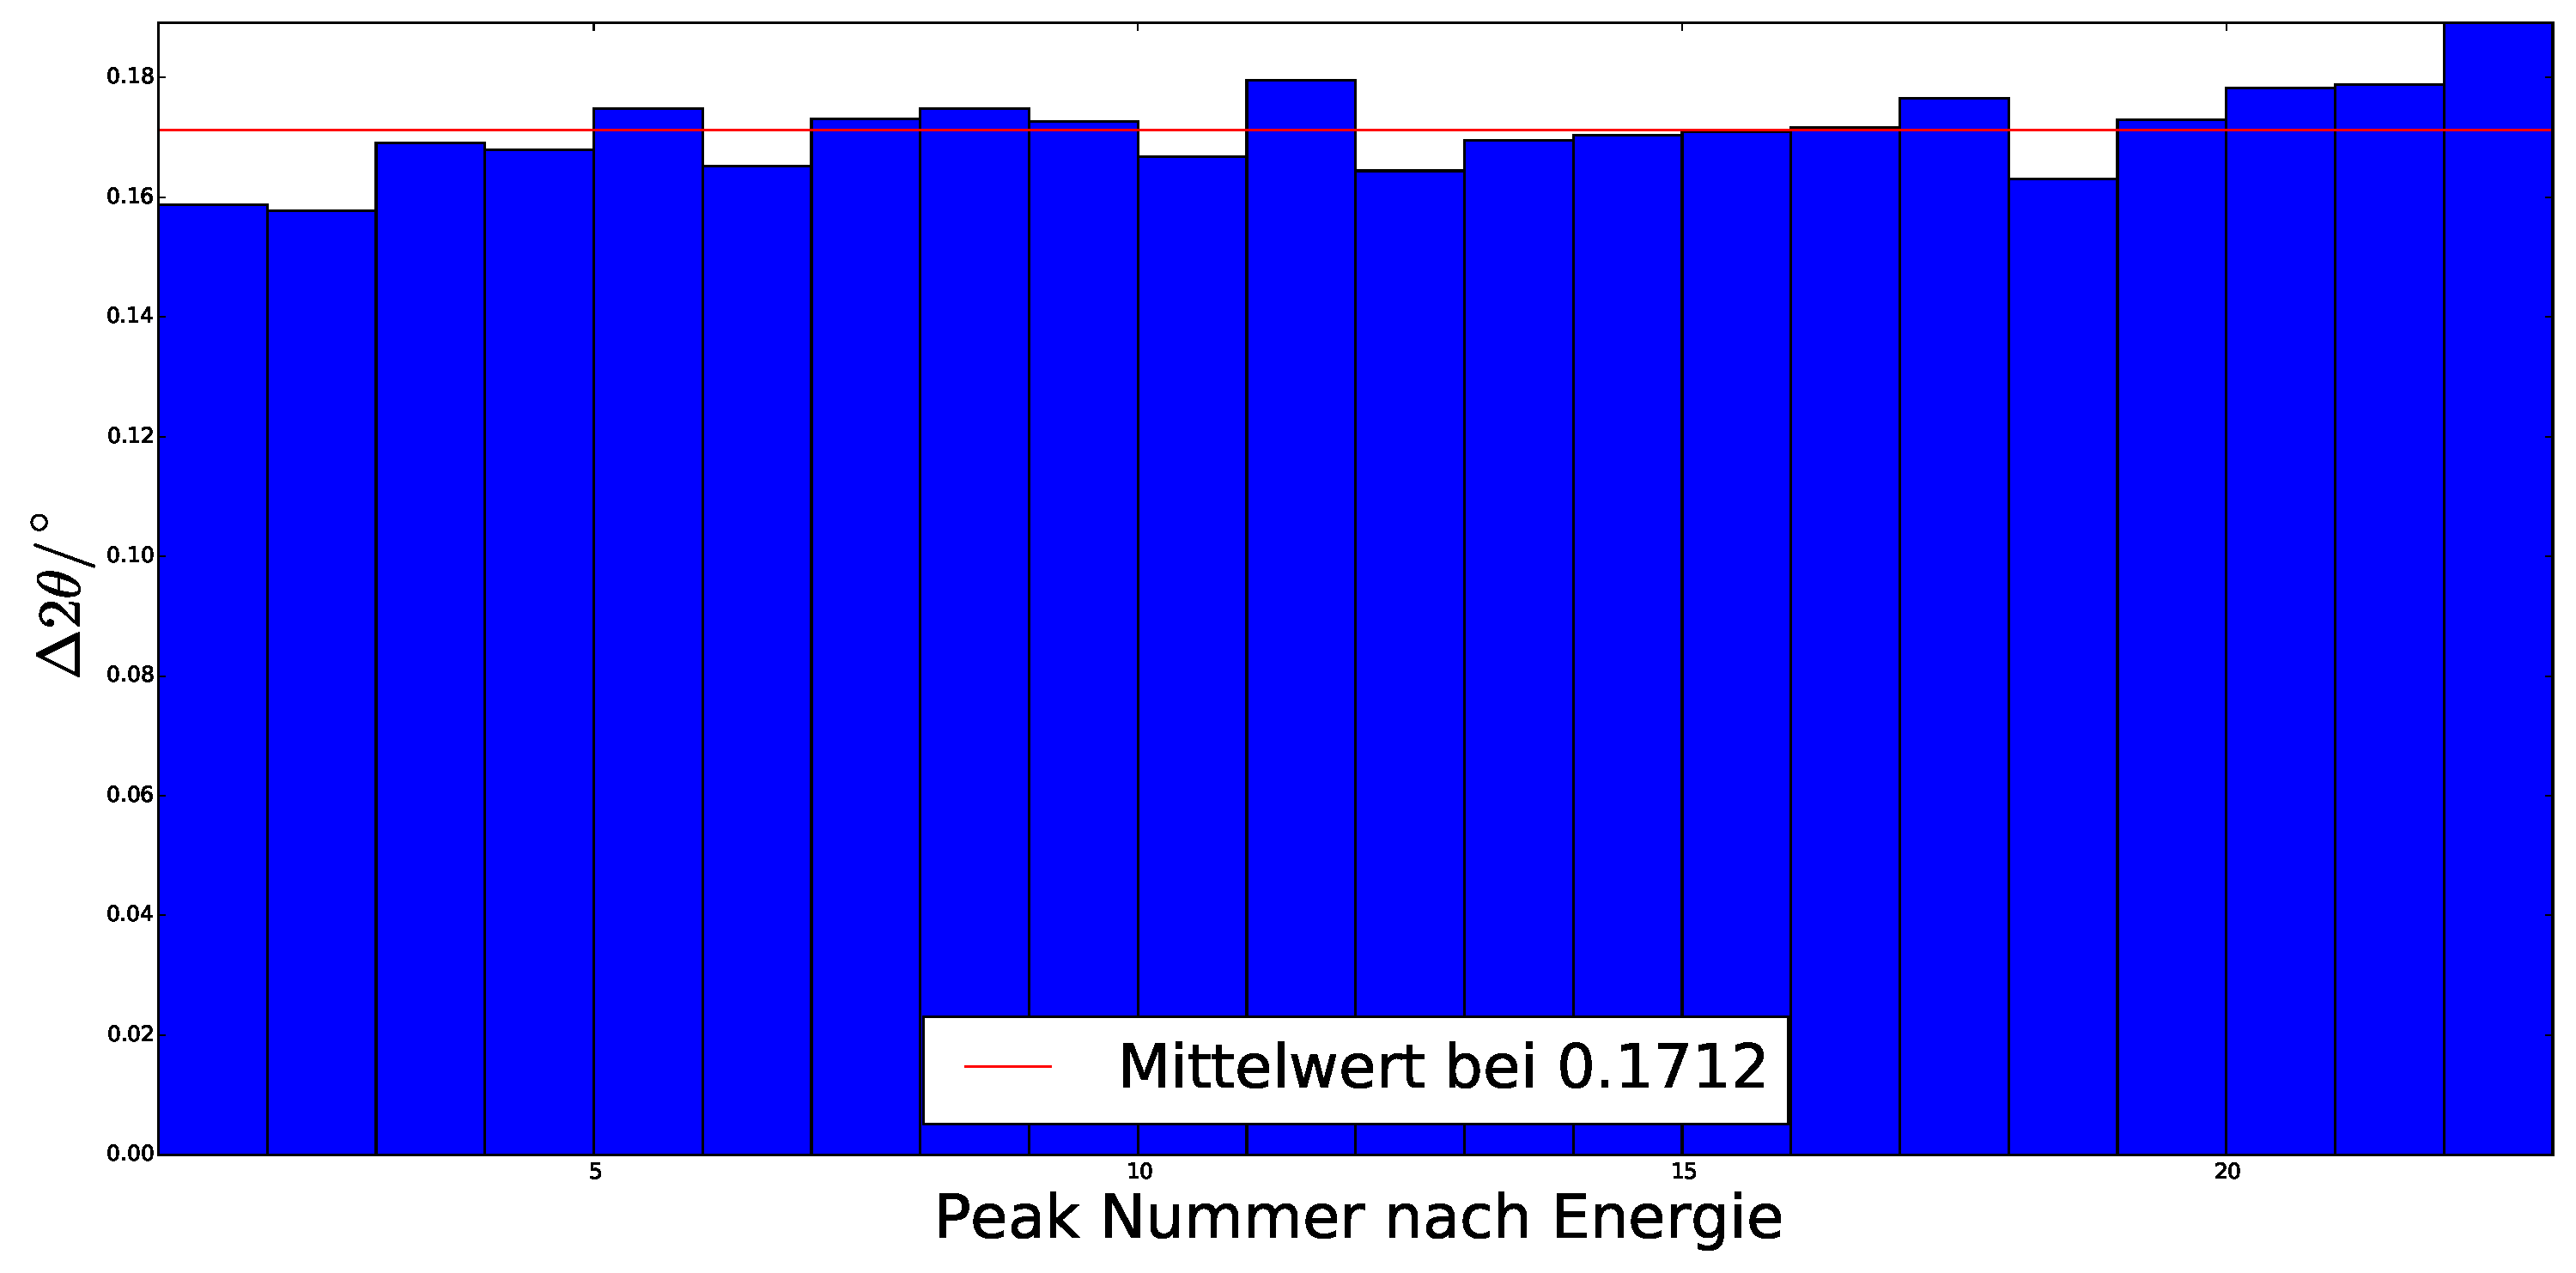
\includegraphics[scale = 0.35]{Differenzplot_pulver_Energie}
   \caption{Peakdifferenzen der Energie nach geordnet} 
  \label{fig:differenzplot_energie}
\end{figure}
\begin{figure}[H]
\begin{minipage}{.49\textwidth}
  \centering
  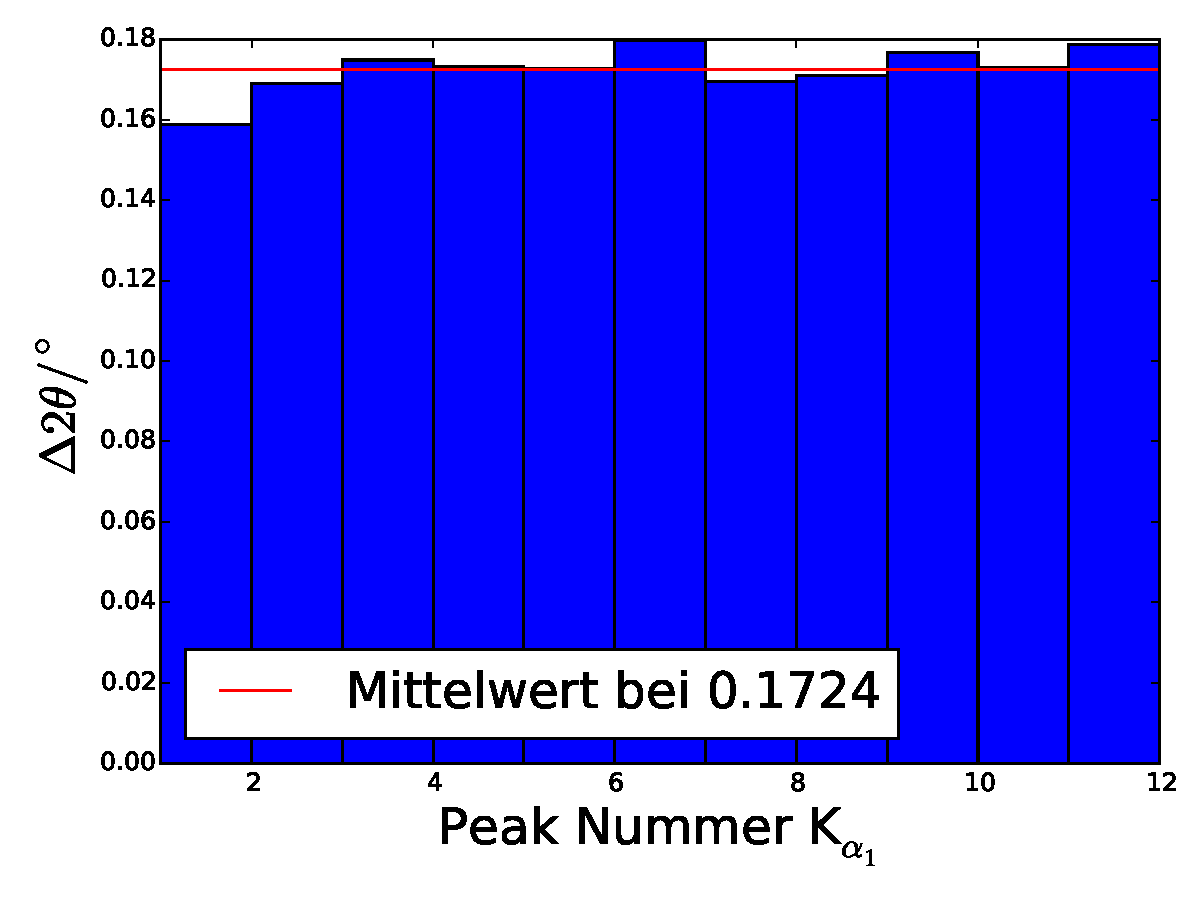
\includegraphics[scale=0.46]{Differenzplot_pulver_K_alpha_1}
  \captionof{figure}{Peakdifferenzen von K$_{\alpha_1}$ der Energie nach geordnet}
  \label{fig:differenzplot_energie_alpha_1}
\end{minipage}
\hspace{0.2cm}
\begin{minipage}{.49\textwidth}
  \centering
  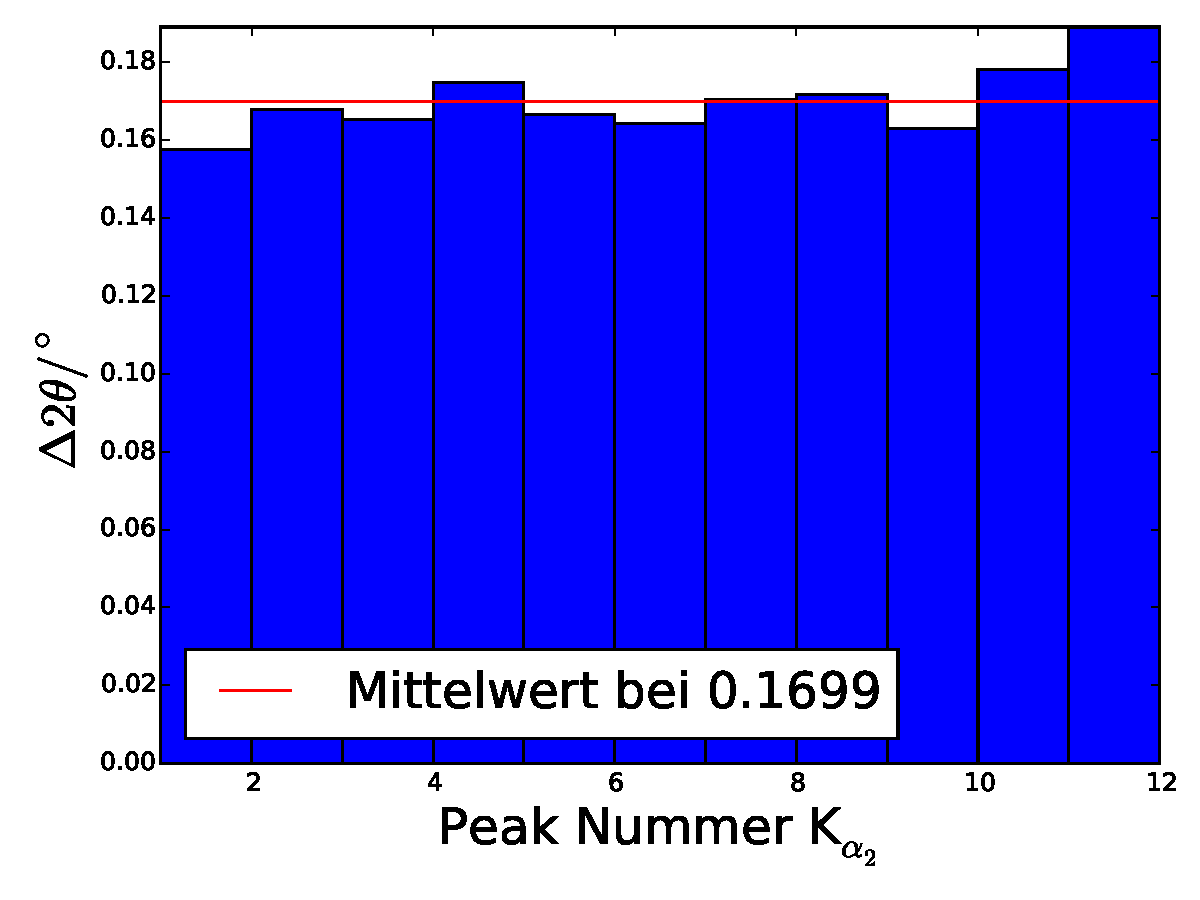
\includegraphics[scale=0.45]{Differenzplot_pulver_K_alpha_2}
  \captionof{figure}{Peakdifferenzen von K$_{\alpha_2}$ der Energie nach geordnet}
  \label{fig:differenzplot_energie_alpha_2}
\end{minipage}
\end{figure}
Man sieht bei allen Plots einen leichten Anstieg der Differenzen der Energien f�r kleine Energiewerte. Es wird trotzdem ein Offset in Form einer Konstanten angenommen. Es ergibt sich damit eine mittlere Abweichung von \SI{0.1712}{\degree}, die haupts�chlich auf einen systematischen Fehler zur�ckzuf�hren ist. Nachdem man die Messdaten um diesen Offset nach rechts verschiebt, stimmt die Lage der Peaks des untersuchten Pulvers bis auf die bereits angesprochene minimale Steigung �berein. Das untersuchte Material kann also mit Siliciumpulver identifiziert werden. Die Herkunft des Offsets ist auf die im Vergleich zur Theorie h�heren gemessenen Energien der K$_{\alpha_1}$ und K$_{\alpha_2}$ Linien in Versuchsteil 3.2.3 zur�ckzuf�hren. Indem man Formel \ref{eqn:bragg_kurze_fassung} nach $\theta$ umstellt, Tabelle \ref{tab:enerige_k}) verwendet und die Winkel mit den Winkeln, welche sich aus den Literaturwerten f�r die Energien ergeben, vergleicht, findet man schlie�lich auch einen Grund f�r die bereits angesprochene minimale Steigung. Nachdem man Formel \ref{eqn:bragg_kurze_fassung} bis zur ersten Ordnung taylort und die Differenz zwischen
\begin{align}
\sin(\theta_{Theorie}) = \frac{hc}{2d_{[nh,nk,nl]} E_{Literatur}}
\end{align}
und
\begin{align}
\sin(\theta_{Messung}) &\approx \frac{hc}{2d_{[nh,nk,nl]} E_{Messung}} \\ \notag
&= \frac{hc}{2d_{[nh,nk,nl]}}\left(\frac{1}{E_{Literatur}}-\frac{1}{E^2_{Literatur}}(E_{Messung}-E_{Literatur})\right)
\end{align}
bildet, findet man den Offset
\begin{align}
\Delta\theta \approx \sin(\theta_{Messung})-\sin(\theta_{Theorie}) \approx \frac{(-1)hc}{2d_{[nh,nk,nl]}E^2_{Literatur}}(E_{Messung}-E_{Literatur})
\end{align}
welcher abh�ngig von d$_{[nh,nk,nl]}$ ist. Bei gro�en Netzebenenabst�nden (kleinen Winkeln $\theta$) ergibt sich ein kleinerer negativer Offset, sowie bei kleinen Netzebenenabst�nden (gr��eren Winkeln $\theta$) ein gr��erer negativer Offset. Die Steigung des Offsets ist gering, da die Unterschiede zwischen den Netzebenenabst�nden gering sind.  Ein konstanter Offset ist deshalb f�r die qualitative Betrachtung ausreichend. Die Netzebenenabst�nde lassen sich aus Formel \ref{eqn:netzebenen} und den in Tabelle \ref{tab:enerige_k} bestimmten Energien bestimmen. Zuvor werden die Ordnung und die Werte h,k,l in der Form [nh,nk,nl] bestimmt, indem man Formel \ref{eqn:d_nh,nk,nl}
\begin{align}
d_{[nh,nk,nl]} = \frac{a}{\sqrt{(nh)^2+(nk)^2+(nl)^2}}
\label{eqn:d_nh,nk,nl}
\end{align}
in Formel \ref{eqn:bragg_kurze_fassung} einsetzt und nach $(nh)^2+(nk)^2+(nl)^2$ umstellt.($a = \SI{5,431020504}{\angstrom}$ ist die Gitterkonstante von Silicium.) Dabei wird auf eine Fehlerrechnung verzichtet.
Es ergibt sich Formel \ref{eqn:(nh)^2+(nk)^2+(nl)^2}.
\begin{align}
(nh)^2+(nk)^2+(nl)^2 = \frac{4E^2a^2}{h^2c^2}\sin^2(\theta)
\label{eqn:(nh)^2+(nk)^2+(nl)^2}
\end{align}
Ob man f�r E die theoretischen Energien oder die experimentell bestimmten Energien aus Tabelle \ref{tab:enerige_k} nimmt, �ndert nichts an den Werten $nh$,$nk$,$nl$. (Aus Symmetriegr�nden $h>k>l$.)
In Tabelle \ref{table:Auswertung_K_alpha_1} und \ref{table:Auswertung_K_alpha_1} werden die so bestimmten Werte $[nh,nk,nl]$, sowie die sich aus Formel \ref{eqn:bragg_kurze_fassung} ergebenden Netzebenenabst�nde d$_{[nh,nk,nl] exp}$ dargestellt und mit den theoretischen Netzebenenabst�nden d$_{[nh,nk,nl] theo}$ aus Formel \ref{eqn:d_nh,nk,nl} verglichen. Die Auswahlregeln f�r Diamantgitter werden dabei beachtet ($h$,$k$,$l$ alle ungerade, oder $h$,$k$,$l$ alle gerade und $h+k+l$ durch 4 teilbar).
\begin{table}[H]
\caption{Auswertung der K$_{\alpha_1}$ Linie}
\centering
\label{table:Auswertung_K_alpha_1}
\begin{tabular}{|c|c|c|c|c|}
\hline  2$\theta_{exp}/^{\circ}$  & d$_{[nh,nk,nl] theo}$ & d$_{[nh,nk,nl] exp}$ & Relative Abweichung/\% & [nh,nk,nl] \\
\hline 28,287 & \SI{3,135601}{\angstrom} & \SI{3,150855}{\angstrom} & 0.486 & [1,1,1]\\
\hline 47,146 & \SI{1,920156}{\angstrom} & \SI{1,925180}{\angstrom} & 0.262 & [2,2,0]\\
\hline 55,963 & \SI{1,637514}{\angstrom} & \SI{1,640995}{\angstrom} & 0.213 & [3,1,1]\\
\hline 68,969 & \SI{1,357755}{\angstrom} & \SI{1,359786}{\angstrom} & 0.150 & [4,0,0]\\
\hline 76,223 & \SI{1,245962}{\angstrom} & \SI{1,247479}{\angstrom} & 0.122 & [3,3,1]\\
\hline 87,875 & \SI{1,108602}{\angstrom} & \SI{1,109590}{\angstrom} & 0.089 & [4,2,2]\\
\hline 94,802 & \SI{1,045200}{\angstrom} & \SI{1,045871}{\angstrom} & 0.064 & [3,3,3]/[5,1,1]\\
\hline 106,565 & \SI{0,960078}{\angstrom} & \SI{0,960458}{\angstrom} & 0.040 & [220]\\
\hline 113,949 & \SI{0,918010}{\angstrom} & \SI{0,918297}{\angstrom} & 0.031 & [531]\\
\hline 127,406 & \SI{0,858720}{\angstrom} & \SI{0,858757}{\angstrom} & 0.004 & [6,2,0]\\
\hline 136,766 & \SI{0,828223}{\angstrom} & \SI{0,828156}{\angstrom} & 0.008 & [5,3,3]\\
\hline 
\end{tabular}
\end{table}
\begin{table}[H]
\caption{Auswertung der K$_{\alpha_2}$ Linie}
\centering
\label{table:Auswertung_K_alpha_2}
\begin{tabular}{|c|c|c|c|c|}
\hline  2$\theta_{exp}/^{\circ}$  & d$_{[nh,nk,nl] theo}$ & d$_{[nh,nk,nl] exp}$ & Relative Abweichung/\% & [nh,nk,nl] \\
\hline 28,363 & \SI{3,135601}{\angstrom} & \SI{3,150912}{\angstrom} & 0.488 & [1,1,1]\\
\hline 47,271 & \SI{1,920156}{\angstrom} & \SI{1,925286}{\angstrom} & 0.267 & [2,2,0]\\
\hline 56,116 & \SI{1,637514}{\angstrom} & \SI{1,640896}{\angstrom} & 0.207 & [3,1,1]\\
\hline 69,167 & \SI{1,357755}{\angstrom} & \SI{1,359801}{\angstrom} & 0.151 & [4,0,0]\\
\hline 76,454 & \SI{1,245962}{\angstrom} & \SI{1,247354}{\angstrom} & 0.112 & [3,3,1]\\
\hline 88,155 & \SI{1,108602}{\angstrom} & \SI{1,109467}{\angstrom} & 0.078 & [4,2,2]\\
\hline 95,111 & \SI{1,045200}{\angstrom} & \SI{1,045871}{\angstrom} & 0.064 & [3,3,3]/[5,1,1]\\
\hline 106,949 & \SI{0,960078}{\angstrom} & \SI{0,960467}{\angstrom} & 0.041 & [220]\\
\hline 114,388 & \SI{0,918010}{\angstrom} & \SI{0,918211}{\angstrom} & 0.022 & [531]\\
\hline 127,985 & \SI{0,858720}{\angstrom} & \SI{0,858763}{\angstrom} &  0.005 & [6,2,0]\\
\hline 137,505 & \SI{0,828223}{\angstrom} & \SI{0,828160}{\angstrom} &  0.008 & [5,3,3]\\
\hline 
\end{tabular}
\end{table}
Man sieht, dass die Abweichungen von den theoretischen Netzebenenabst�nden bei unter einem halben Prozent liegen. Die Resultate best�tigen, dass es sich um Siliciumpulver handelt.
Zuletzt sollen die Korngr��en mithilfe der Scherrer-Gleichung abgesch�tzt werden. Mit Gleichung \ref{eqn:scherrer_korngroesse} wird die Korngr��e aus FWHM und den Energien der K$_{\alpha}$-Linien bestimmt. Auf eine Fehlerrechung wird aufgrund der geringen Genauigkeit des Scherrer-Formfaktors verzichtet.
\begin{table}[H]
\caption{Auswertung der K$_{\alpha_1}$ Linie}
\centering
\label{table:korngroesse_K_alpha_1}
\begin{tabular}{|c|c|c|}
\hline  2$\theta_{exp}/^{\circ}$  & FWHM/$^{\circ}$ & B/\AA{}\\
\hline 28,287 & 0.0256 & 58,222 \\
\hline 47,146 & 0.0256 & 61,597 \\
\hline 55,963 & 0.0384 & 42,620 \\
\hline 68,969 & 0.0384 & 45,663 \\
\hline 76,223 & 0.0320 & 57,402 \\
\hline 87,875 & 0.0256 & 78,401 \\
\hline 94,802 & 0.0512 & 41,707 \\
\hline 106,565 & 0.0512 & 47,216 \\
\hline 113,949 & 0.0705 & 37,666 \\
\hline 127,406 & 0.0769 & 42,482 \\
\hline 136,766 & 0.0640 & 61,294 \\
\hline
\end{tabular} 
\end{table}
\begin{table}[H]
\caption{Auswertung der K$_{\alpha_2}$ Linie}
\centering
\label{table:korngroesse_K_alpha_2}
\begin{tabular}{|c|c|c|}
\hline  2$\theta_{exp}/^{\circ}$  & FWHM/$^{\circ}$ & B/\AA{}\\
\hline 28,363 & 0.0320 & 46,701 \\
\hline 47,271 & 0.0192 & 82,372 \\
\hline 56,116 & 0.0320 & 51,308 \\
\hline 69,167 & 0.0256 & 68,744 \\
\hline 76,454 & 0.0256 & 72,045 \\
\hline 88,155 & 0.0320 & 63,028 \\
\hline 95,111 & 0.0513 & 41,933 \\
\hline 106,949 & 0.0577 & 42,262 \\
\hline 114,388 & 0.0641 & 41,790 \\
\hline 127,985 & 0.0513 & 64,538 \\
\hline 137,505 & 0.0897 & 44,599 \\
\hline
\end{tabular} 
\end{table}
Die Korngr��en k�nnen in der Gr��enordnung von 38\AA{} bis 82\AA{} abgesch�tzt werden. 
\begin{sidewaysfigure}
\centering
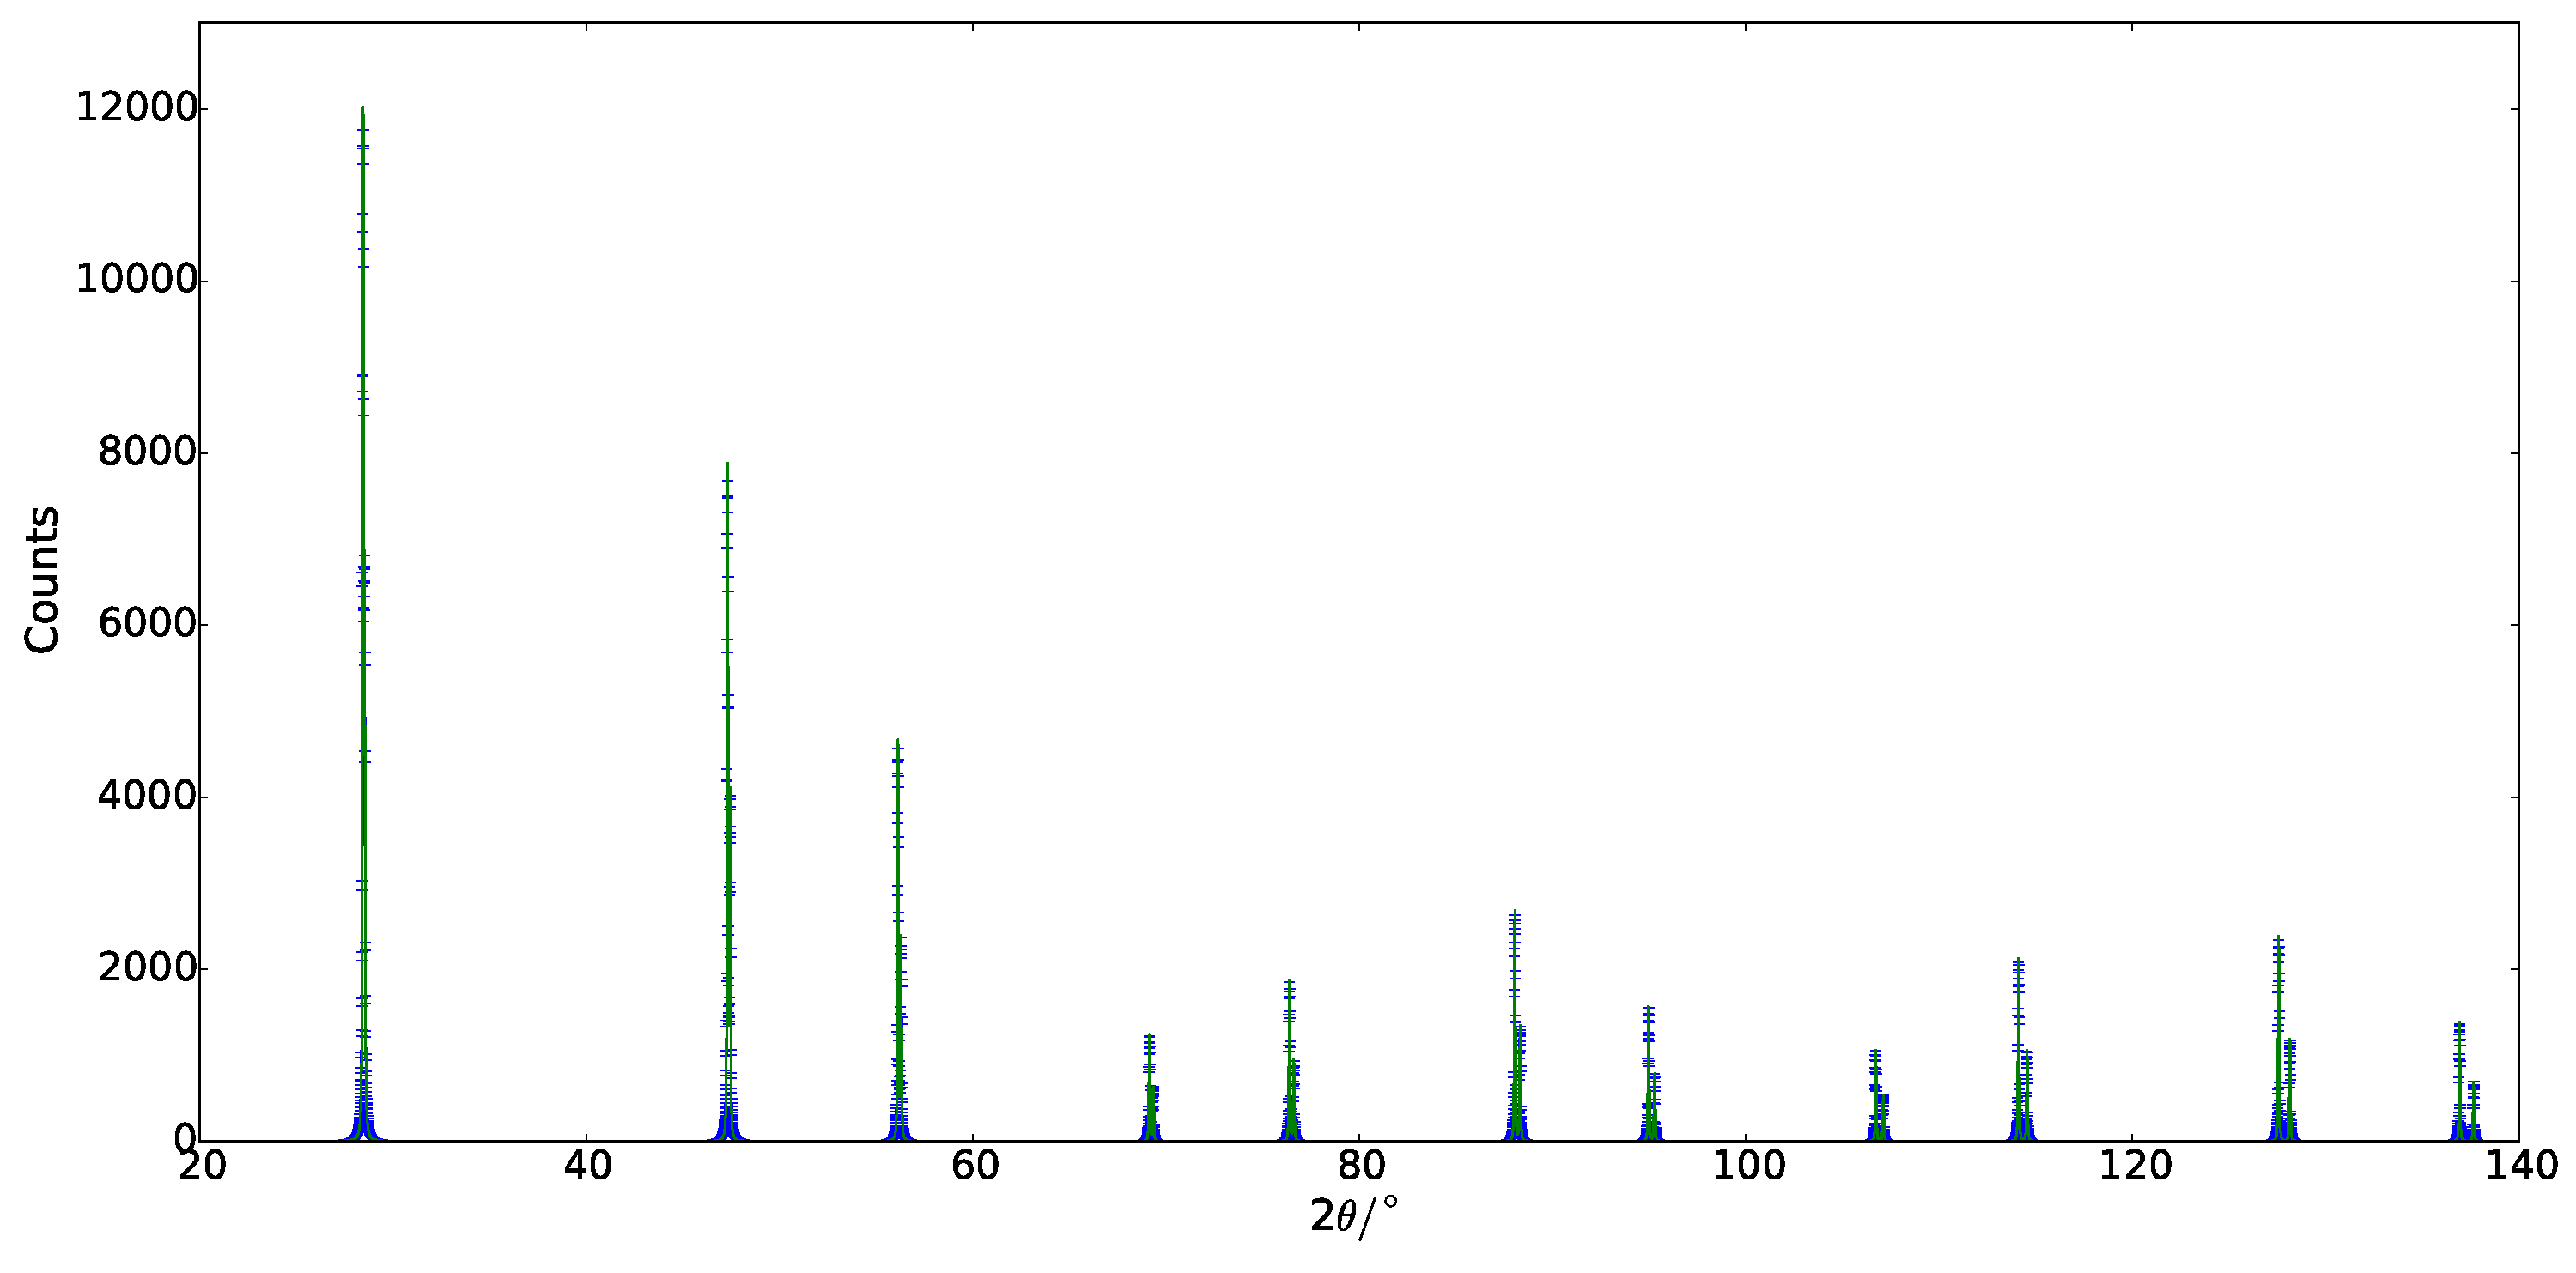
\includegraphics[width = 1.0\textwidth, height = 0.7\textwidth]{messung_pulver_ges}
\caption{Diffraktogramm der Pulverprobe}
\label{fig:diffr_pulver}
\end{sidewaysfigure}
\begin{sidewaysfigure}
\centering
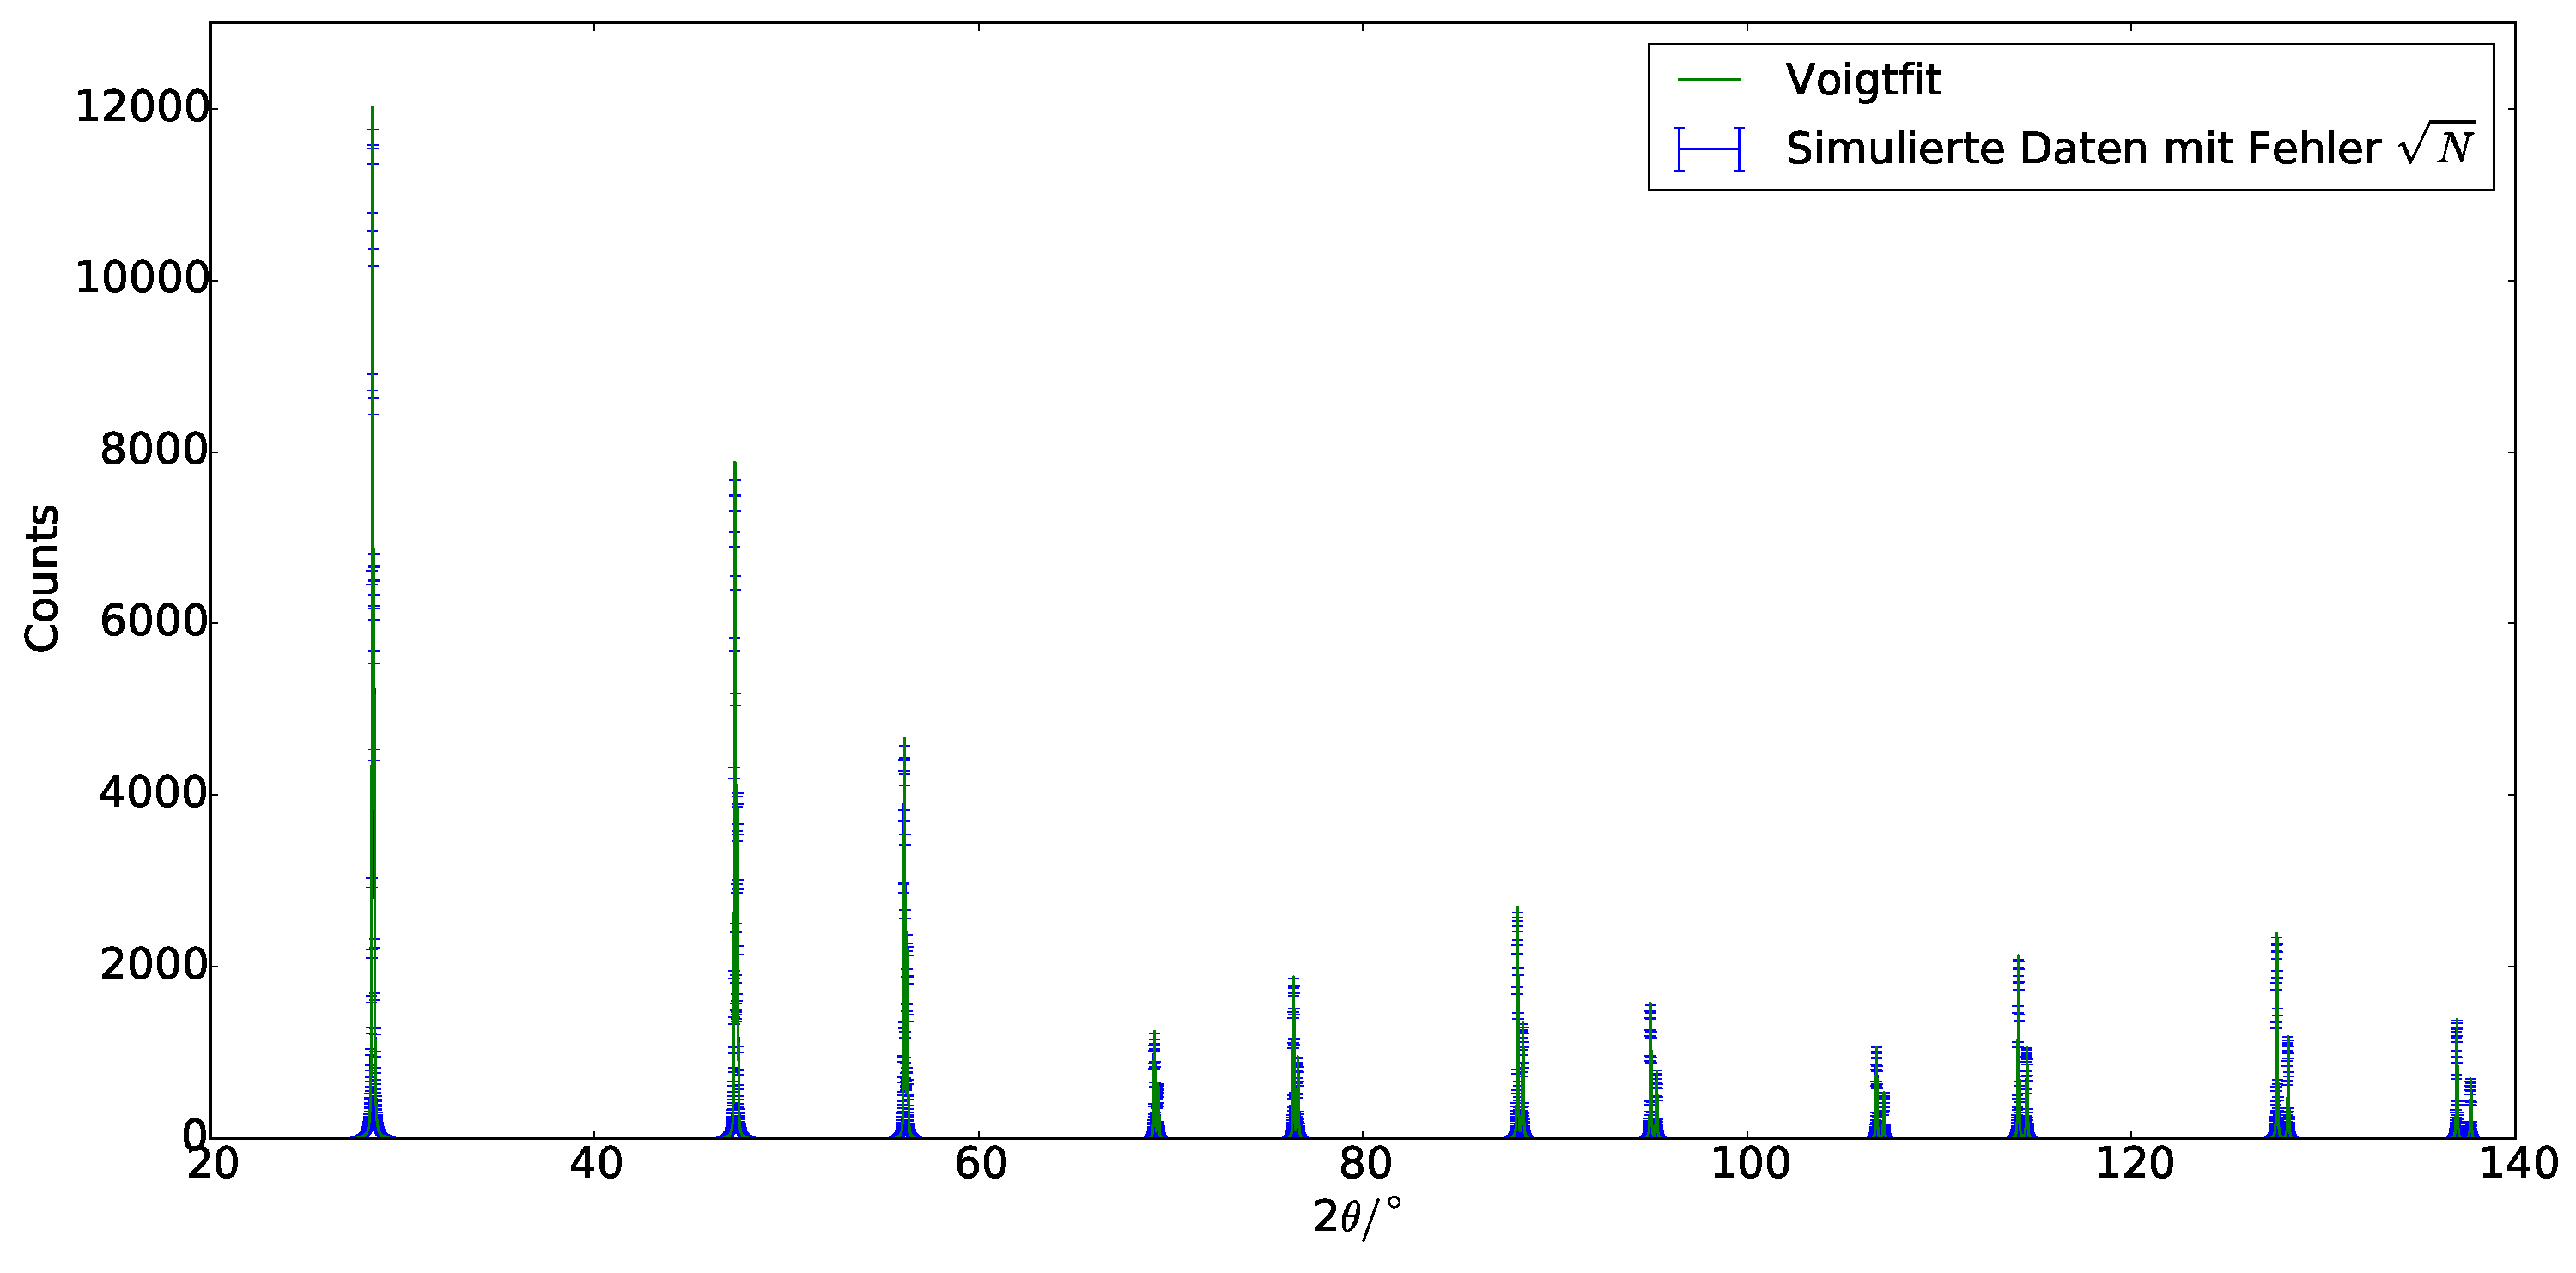
\includegraphics[width = 1.0\textwidth, height = 0.7\textwidth]{Simulation_Siliciumpulver_ges}
\caption{Diffraktogramm der Siliciumsimulation}
\label{fig:diffr_sil_sim}
\end{sidewaysfigure}
\begin{sidewaysfigure}
\centering
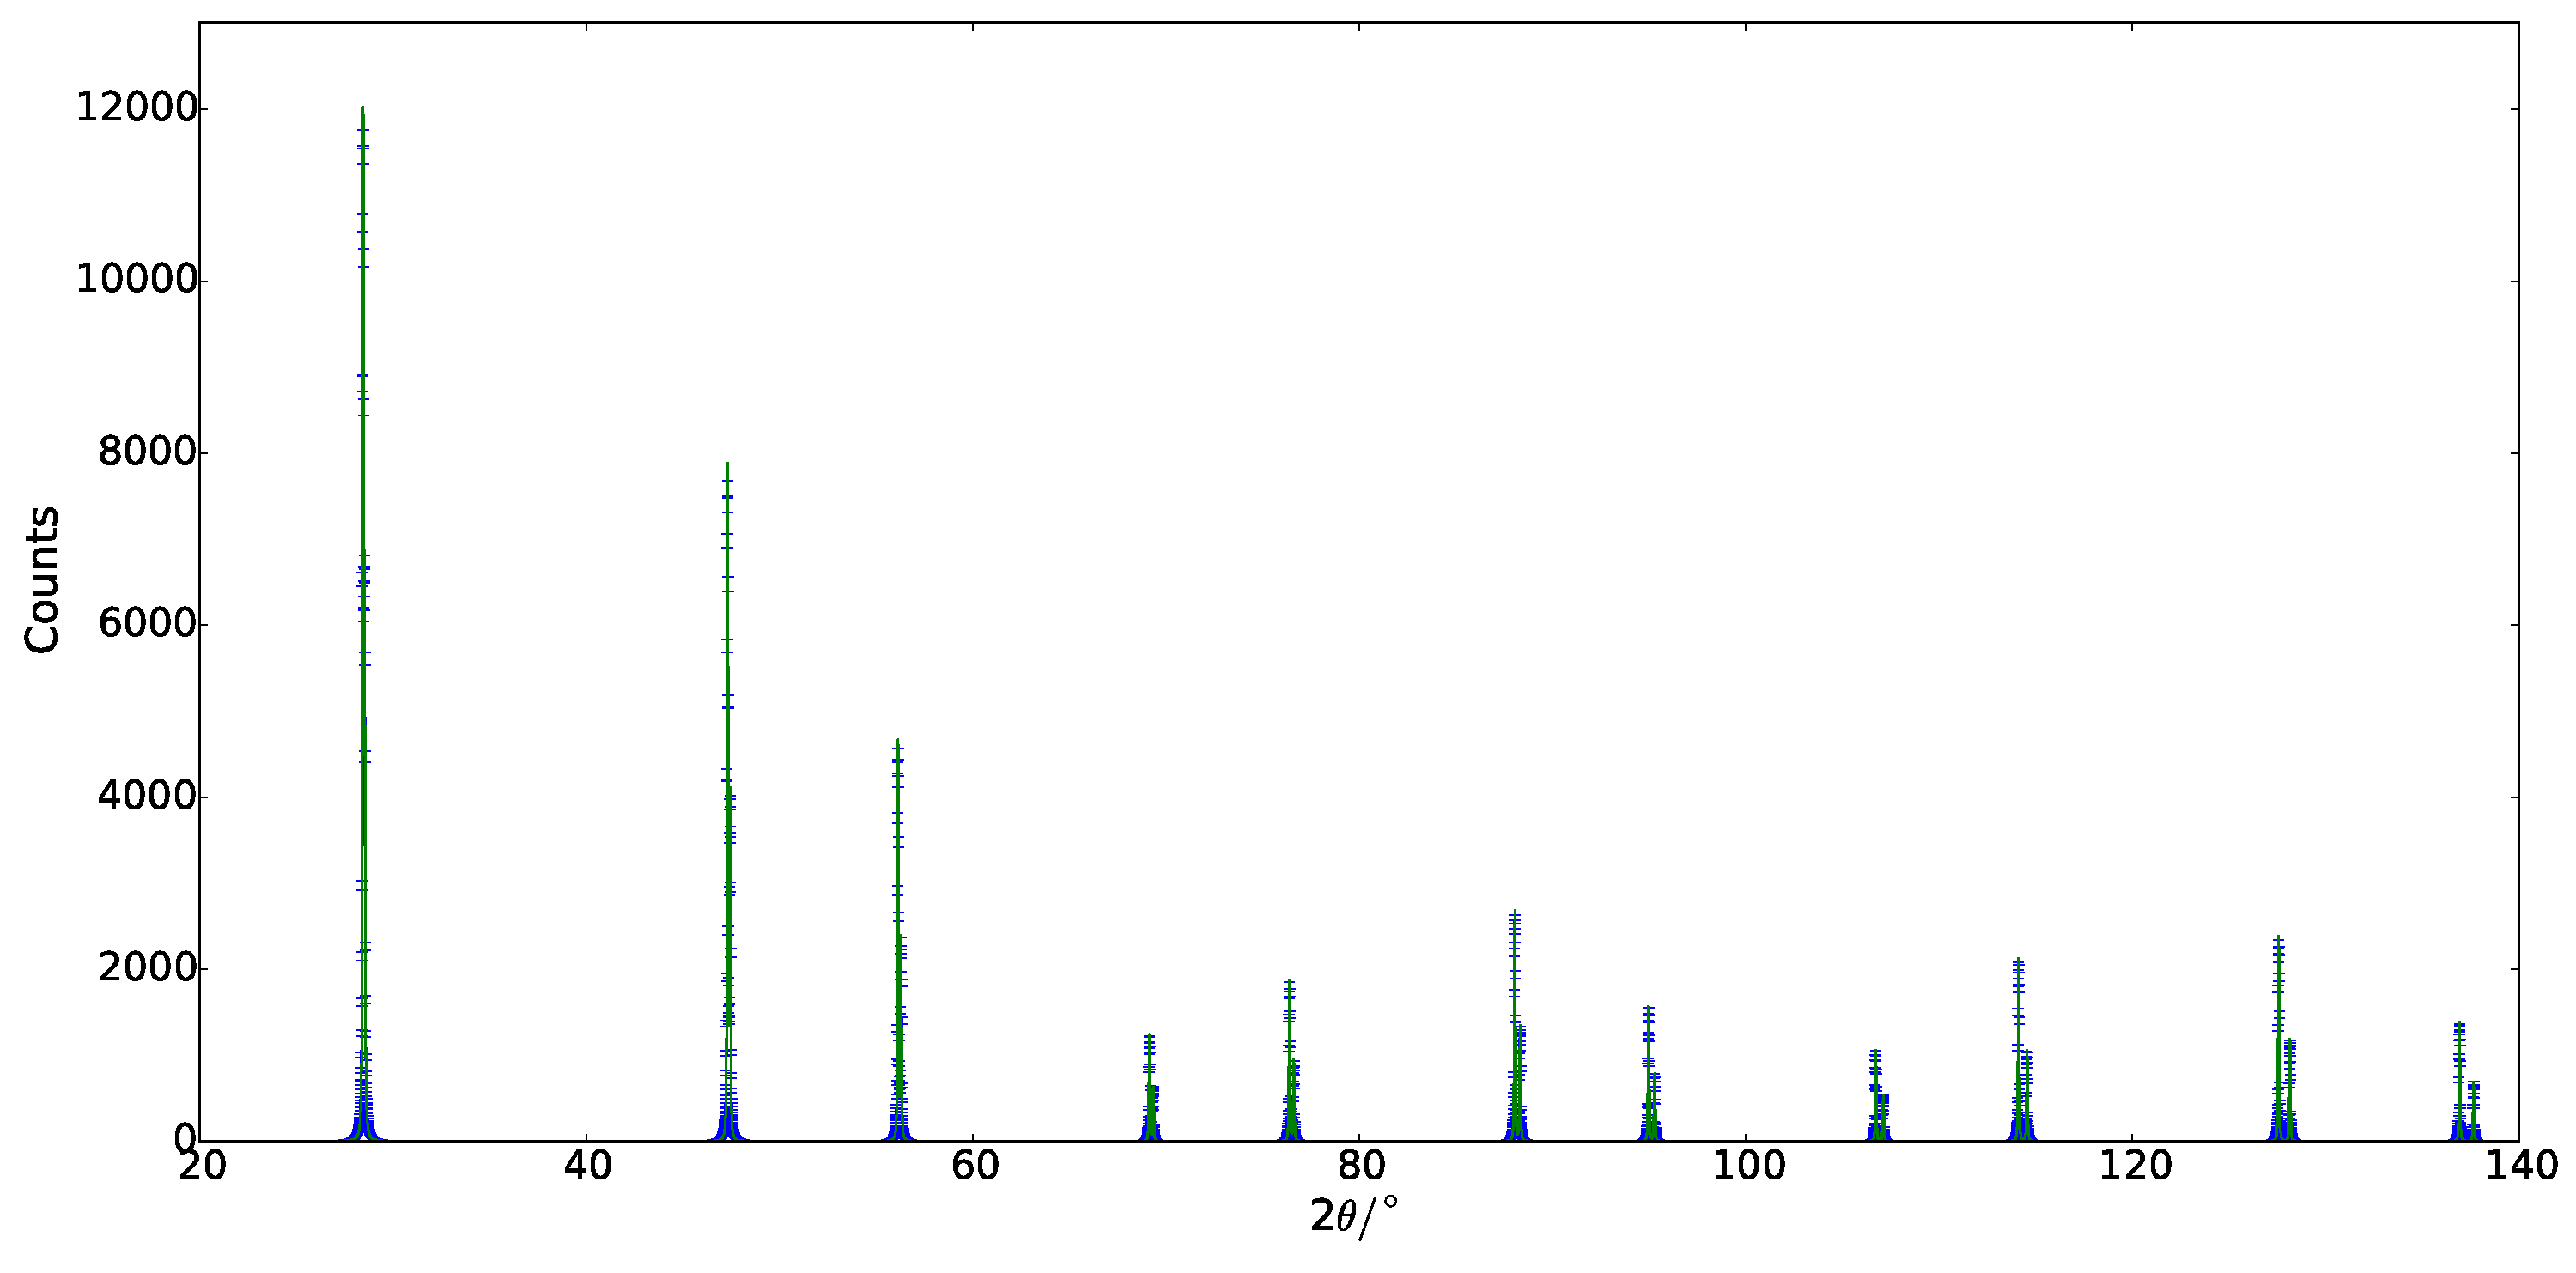
\includegraphics[width = 1.0\textwidth, height = 0.7\textwidth]{messung_pulver_ges}
\caption{Diffraktogramm der Germaniumsimulation}
\label{fig:diffr_ger_sim}
\end{sidewaysfigure}

\section{Conclusion}
%im fazit nochmal alles zusammenfassen und den verlauf der messung absch�tzen
%gravierende sytematische probleme bei den messungen nochmal betonen und die wertigkeit unserer ergebnisse einordnen

In the first part of the experiment the 39 peaks of the nH$_3$ spectrum where measured and there relative absorption coefficients where calculated. In the second part the quadrupole moment where determined with a value of 5.02(9), with a deviation of 17.53\%. In the last part the broadening of the peaks according to the pressure was determined with 28 witch is a good measurement. 



%\bibliography{ref}

\end{document}